\documentclass[oneside]{memoir}
\usepackage{lmodern}
\usepackage{amssymb,amsmath}
\usepackage{ifxetex,ifluatex}
\usepackage{fixltx2e} % provides \textsubscript
\ifnum 0\ifxetex 1\fi\ifluatex 1\fi=0 % if pdftex
  \usepackage[T1]{fontenc}
  \usepackage[utf8]{inputenc}
\else % if luatex or xelatex
  \ifxetex
    \usepackage{mathspec}
  \else
    \usepackage{fontspec}
  \fi
  \defaultfontfeatures{Ligatures=TeX,Scale=MatchLowercase}
\fi
% use upquote if available, for straight quotes in verbatim environments
\IfFileExists{upquote.sty}{\usepackage{upquote}}{}
% use microtype if available
\IfFileExists{microtype.sty}{%
\usepackage{microtype}
\UseMicrotypeSet[protrusion]{basicmath} % disable protrusion for tt fonts
}{}
\usepackage[margin=1in]{geometry}
\usepackage{hyperref}
\hypersetup{unicode=true,
            pdftitle={Introduction to Data Visualization},
            pdfauthor={LTC Melanie Vinton},
            pdfborder={0 0 0},
            breaklinks=true}
\urlstyle{same}  % don't use monospace font for urls
\usepackage{color}
\usepackage{fancyvrb}
\newcommand{\VerbBar}{|}
\newcommand{\VERB}{\Verb[commandchars=\\\{\}]}
\DefineVerbatimEnvironment{Highlighting}{Verbatim}{commandchars=\\\{\}}
% Add ',fontsize=\small' for more characters per line
\usepackage{framed}
\definecolor{shadecolor}{RGB}{248,248,248}
\newenvironment{Shaded}{\begin{snugshade}}{\end{snugshade}}
\newcommand{\KeywordTok}[1]{\textcolor[rgb]{0.13,0.29,0.53}{\textbf{#1}}}
\newcommand{\DataTypeTok}[1]{\textcolor[rgb]{0.13,0.29,0.53}{#1}}
\newcommand{\DecValTok}[1]{\textcolor[rgb]{0.00,0.00,0.81}{#1}}
\newcommand{\BaseNTok}[1]{\textcolor[rgb]{0.00,0.00,0.81}{#1}}
\newcommand{\FloatTok}[1]{\textcolor[rgb]{0.00,0.00,0.81}{#1}}
\newcommand{\ConstantTok}[1]{\textcolor[rgb]{0.00,0.00,0.00}{#1}}
\newcommand{\CharTok}[1]{\textcolor[rgb]{0.31,0.60,0.02}{#1}}
\newcommand{\SpecialCharTok}[1]{\textcolor[rgb]{0.00,0.00,0.00}{#1}}
\newcommand{\StringTok}[1]{\textcolor[rgb]{0.31,0.60,0.02}{#1}}
\newcommand{\VerbatimStringTok}[1]{\textcolor[rgb]{0.31,0.60,0.02}{#1}}
\newcommand{\SpecialStringTok}[1]{\textcolor[rgb]{0.31,0.60,0.02}{#1}}
\newcommand{\ImportTok}[1]{#1}
\newcommand{\CommentTok}[1]{\textcolor[rgb]{0.56,0.35,0.01}{\textit{#1}}}
\newcommand{\DocumentationTok}[1]{\textcolor[rgb]{0.56,0.35,0.01}{\textbf{\textit{#1}}}}
\newcommand{\AnnotationTok}[1]{\textcolor[rgb]{0.56,0.35,0.01}{\textbf{\textit{#1}}}}
\newcommand{\CommentVarTok}[1]{\textcolor[rgb]{0.56,0.35,0.01}{\textbf{\textit{#1}}}}
\newcommand{\OtherTok}[1]{\textcolor[rgb]{0.56,0.35,0.01}{#1}}
\newcommand{\FunctionTok}[1]{\textcolor[rgb]{0.00,0.00,0.00}{#1}}
\newcommand{\VariableTok}[1]{\textcolor[rgb]{0.00,0.00,0.00}{#1}}
\newcommand{\ControlFlowTok}[1]{\textcolor[rgb]{0.13,0.29,0.53}{\textbf{#1}}}
\newcommand{\OperatorTok}[1]{\textcolor[rgb]{0.81,0.36,0.00}{\textbf{#1}}}
\newcommand{\BuiltInTok}[1]{#1}
\newcommand{\ExtensionTok}[1]{#1}
\newcommand{\PreprocessorTok}[1]{\textcolor[rgb]{0.56,0.35,0.01}{\textit{#1}}}
\newcommand{\AttributeTok}[1]{\textcolor[rgb]{0.77,0.63,0.00}{#1}}
\newcommand{\RegionMarkerTok}[1]{#1}
\newcommand{\InformationTok}[1]{\textcolor[rgb]{0.56,0.35,0.01}{\textbf{\textit{#1}}}}
\newcommand{\WarningTok}[1]{\textcolor[rgb]{0.56,0.35,0.01}{\textbf{\textit{#1}}}}
\newcommand{\AlertTok}[1]{\textcolor[rgb]{0.94,0.16,0.16}{#1}}
\newcommand{\ErrorTok}[1]{\textcolor[rgb]{0.64,0.00,0.00}{\textbf{#1}}}
\newcommand{\NormalTok}[1]{#1}
\usepackage{longtable,booktabs}
\usepackage{graphicx,grffile}
\makeatletter
\def\maxwidth{\ifdim\Gin@nat@width>\linewidth\linewidth\else\Gin@nat@width\fi}
\def\maxheight{\ifdim\Gin@nat@height>\textheight\textheight\else\Gin@nat@height\fi}
\makeatother
% Scale images if necessary, so that they will not overflow the page
% margins by default, and it is still possible to overwrite the defaults
% using explicit options in \includegraphics[width, height, ...]{}
\setkeys{Gin}{width=\maxwidth,height=\maxheight,keepaspectratio}
\IfFileExists{parskip.sty}{%
\usepackage{parskip}
}{% else
\setlength{\parindent}{0pt}
\setlength{\parskip}{6pt plus 2pt minus 1pt}
}
\setlength{\emergencystretch}{3em}  % prevent overfull lines
\providecommand{\tightlist}{%
  \setlength{\itemsep}{0pt}\setlength{\parskip}{0pt}}
\setcounter{secnumdepth}{5}
% Redefines (sub)paragraphs to behave more like sections
\ifx\paragraph\undefined\else
\let\oldparagraph\paragraph
\renewcommand{\paragraph}[1]{\oldparagraph{#1}\mbox{}}
\fi
\ifx\subparagraph\undefined\else
\let\oldsubparagraph\subparagraph
\renewcommand{\subparagraph}[1]{\oldsubparagraph{#1}\mbox{}}
\fi

%%% Use protect on footnotes to avoid problems with footnotes in titles
\let\rmarkdownfootnote\footnote%
\def\footnote{\protect\rmarkdownfootnote}

%%% Change title format to be more compact
\usepackage{titling}

% Create subtitle command for use in maketitle
\newcommand{\subtitle}[1]{
  \posttitle{
    \begin{center}\large#1\end{center}
    }
}

\setlength{\droptitle}{-2em}
  \title{Introduction to Data Visualization}
  \pretitle{\vspace{\droptitle}\centering\huge}
  \posttitle{\par}
  \author{LTC Melanie Vinton}
  \preauthor{\centering\large\emph}
  \postauthor{\par}
  \predate{\centering\large\emph}
  \postdate{\par}
  \date{2017-11-09}

\usepackage{booktabs}
\usepackage{amsthm}
\makeatletter
\def\thm@space@setup{%
  \thm@preskip=8pt plus 2pt minus 4pt
  \thm@postskip=\thm@preskip
}
\makeatother

\usepackage{amsthm}
\newtheorem{theorem}{Theorem}[chapter]
\newtheorem{lemma}{Lemma}[chapter]
\theoremstyle{definition}
\newtheorem{definition}{Definition}[chapter]
\newtheorem{corollary}{Corollary}[chapter]
\newtheorem{proposition}{Proposition}[chapter]
\theoremstyle{definition}
\newtheorem{example}{Example}[chapter]
\theoremstyle{definition}
\newtheorem{exercise}{Exercise}[chapter]
\theoremstyle{remark}
\newtheorem*{remark}{Remark}
\newtheorem*{solution}{Solution}
\begin{document}
\maketitle

{
\setcounter{tocdepth}{1}
\tableofcontents
}
\chapter{Visualization Module Intro}\label{visualization-module-intro}

\textbf{First, restart your R session.}

\href{https://www.youtube.com/watch?v=jbkSRLYSojo}{Motivation}

The purpose of visualization is improve or reinforce human cognition of
abstract data.

This module is an introduction to visualization in R using the
\textbf{ggplot2} package. Many of the most impressive visualizations
seen today are made in R with packages like ggplot2.

Here's some examples:
\url{http://www.r-graph-gallery.com/portfolio/ggplot2-package}

Some elements of this module use the following reference:
\url{http://jcyhong.github.io/ggplot_demo.html}

\chapter{ggplot2 Package}\label{ggplot2-package}

The \textbf{ggplot2} package is based on the grammar of graphics, which
breaks graphics into parts which are controlled separately and combined.

\begin{itemize}
\item
  Plots are constructed in layers, which can be more intuitive.
\item
  This package is among the most useful and widely used for
  visualization in R, created by Hadley Wickham.
\item
  There are plotting functions available in base R but \textbf{ggplot2}
  provides a powerful, intuitive framework for creating and customizing
  visualizations.
\end{itemize}

\section{Layering}\label{layering}

Every graph has the same basic components:

\begin{enumerate}
\def\labelenumi{\arabic{enumi}.}
\tightlist
\item
  Data
\end{enumerate}

\begin{itemize}
\tightlist
\item
  usually a data frame
\end{itemize}

\begin{enumerate}
\def\labelenumi{\arabic{enumi}.}
\setcounter{enumi}{1}
\tightlist
\item
  Aesthetic mapping
\end{enumerate}

\begin{itemize}
\tightlist
\item
  how variables in the data frame map to visual objects on the graph
\item
  objects (or aesthetics) to map to include x-axis, y-axis, size, shape,
  color, transparency
\item
  specified with the \texttt{aes()} function
\end{itemize}

\begin{enumerate}
\def\labelenumi{\arabic{enumi}.}
\setcounter{enumi}{2}
\tightlist
\item
  Geoms that represent data points visually.\\
\end{enumerate}

\begin{itemize}
\tightlist
\item
  specifies the type of plot
\item
  geom = geometric object
\item
  examples (see the cheatsheet!): \texttt{geom\_line()},
  \texttt{geom\_point()}, \texttt{geom\_bar()},
  \texttt{geom\_histogram()}
\end{itemize}

\section{Packages}\label{packages}

First, lets install the packages we will use in this module.

\begin{Shaded}
\begin{Highlighting}[]
\KeywordTok{library}\NormalTok{(ggplot2)}
\KeywordTok{library}\NormalTok{(RColorBrewer)}
\KeywordTok{library}\NormalTok{(plyr)}
\KeywordTok{library}\NormalTok{(dplyr)}
\KeywordTok{library}\NormalTok{(lubridate)}
\KeywordTok{library}\NormalTok{(scales)}
\KeywordTok{library}\NormalTok{(plotly)}
\end{Highlighting}
\end{Shaded}

\section{References}\label{references}

Some useful references include:

\begin{itemize}
\item
  \url{http://www.cookbook-r.com}
\item
  \url{http://ggplot2.tidyverse.org/reference/}
\item
  \url{https://www.rstudio.com/resources/cheatsheets/}
\item
  ``R Graphics Cookbook'' by Winston Chang (PDF can be found online at
  \url{http://ase.tufts.edu/bugs/guide/assets/R\%20Graphics\%20Cookbook.pdf})
\item
  \url{http://www.google.com}
\end{itemize}

\chapter{Scatterplots}\label{scatterplots}

A scatterplot displays two variables from a data set. It is often used
to explore the relationship between those variables. You can also add
variables to the visualization with different colors, shapes, and sizes
of the dots.

\section{Cars Data}\label{cars-data}

We will start with a data set of 32 cars and 11 performance and design
features.

\begin{itemize}
\item
  This data was taken from a 1974 issue of Motor Trend magazine and is
  built into base R as a dataframe called ``mtcars''.
\item
  It is often used for educational or demonstration purposes.
\item
  We will read in the data from a CSV because that is the way you would
  handle data in the real world.
\end{itemize}

\begin{Shaded}
\begin{Highlighting}[]
\NormalTok{cars <-}\StringTok{ }\KeywordTok{read.csv}\NormalTok{(}\StringTok{"mtcars.csv"}\NormalTok{, }\DataTypeTok{stringsAsFactors =} \OtherTok{FALSE}\NormalTok{)}
\end{Highlighting}
\end{Shaded}

\begin{Shaded}
\begin{Highlighting}[]
\KeywordTok{head}\NormalTok{(cars)}
\end{Highlighting}
\end{Shaded}

\begin{verbatim}
##                 car  mpg cyl disp  hp drat    wt  qsec vs am gear carb
## 1         Mazda RX4 21.0   6  160 110 3.90 2.620 16.46  0  1    4    4
## 2     Mazda RX4 Wag 21.0   6  160 110 3.90 2.875 17.02  0  1    4    4
## 3        Datsun 710 22.8   4  108  93 3.85 2.320 18.61  1  1    4    1
## 4    Hornet 4 Drive 21.4   6  258 110 3.08 3.215 19.44  1  0    3    1
## 5 Hornet Sportabout 18.7   8  360 175 3.15 3.440 17.02  0  0    3    2
## 6           Valiant 18.1   6  225 105 2.76 3.460 20.22  1  0    3    1
\end{verbatim}

To get the variable descriptions, call the ``mtcars'' dataset in help.

\begin{Shaded}
\begin{Highlighting}[]
\NormalTok{?mtcars}
\end{Highlighting}
\end{Shaded}

\section{Scatterplot}\label{scatterplot}

Let's create a scatterplot of miles per gallon (mpg) versus engine size
(disp).

The first step is to initialize our plot using the \texttt{ggplot()}
function. This creates a coordinate system that we will then add layers
to. We identify the data set to use with the ``data'' parameter and map
the x and y aesthetics with \texttt{aes()}.

\begin{Shaded}
\begin{Highlighting}[]
\KeywordTok{ggplot}\NormalTok{(}\DataTypeTok{data =}\NormalTok{ cars, }\KeywordTok{aes}\NormalTok{(}\DataTypeTok{x =}\NormalTok{ mpg, }\DataTypeTok{y =}\NormalTok{ disp))}
\end{Highlighting}
\end{Shaded}

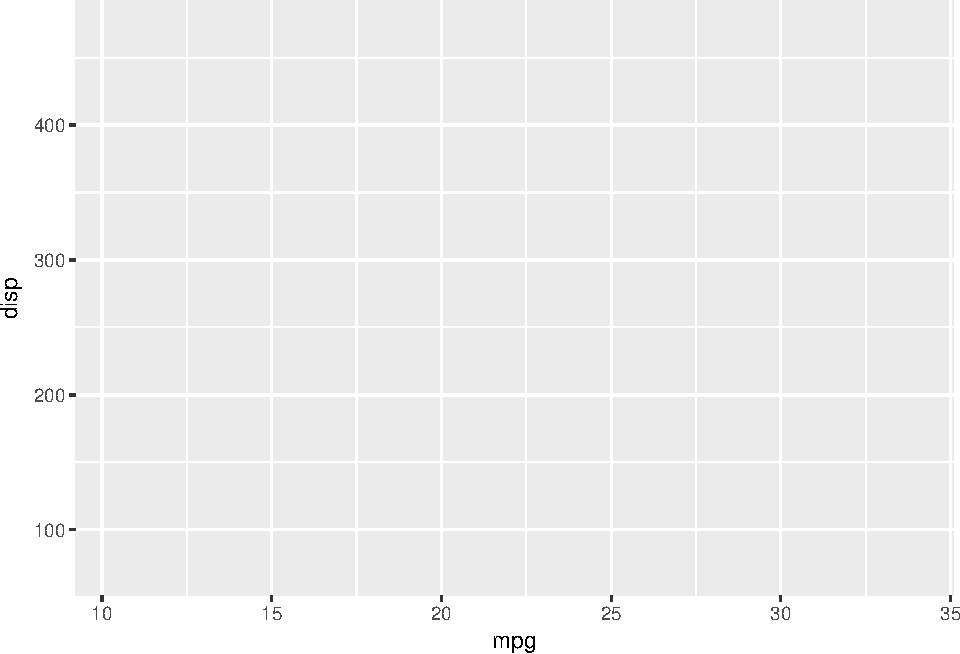
\includegraphics{visualization_files/figure-latex/unnamed-chunk-5-1.pdf}

Notice that R automatically adds the variable names to the axes and has
a default look for the axis lines and background. We will go over how to
customize those later.

Now we will specify the geometric object we want to see on the plot, in
this case points, using the \texttt{geom\_point} function.

Use a ``+'' sign to add the next layer. Be sure it is at the \emph{end}
of the previous line!

\begin{Shaded}
\begin{Highlighting}[]
\KeywordTok{ggplot}\NormalTok{(}\DataTypeTok{data =}\NormalTok{ cars, }\KeywordTok{aes}\NormalTok{(}\DataTypeTok{x =}\NormalTok{ mpg, }\DataTypeTok{y =}\NormalTok{ disp)) }\OperatorTok{+}
\StringTok{  }\KeywordTok{geom_point}\NormalTok{()}
\end{Highlighting}
\end{Shaded}

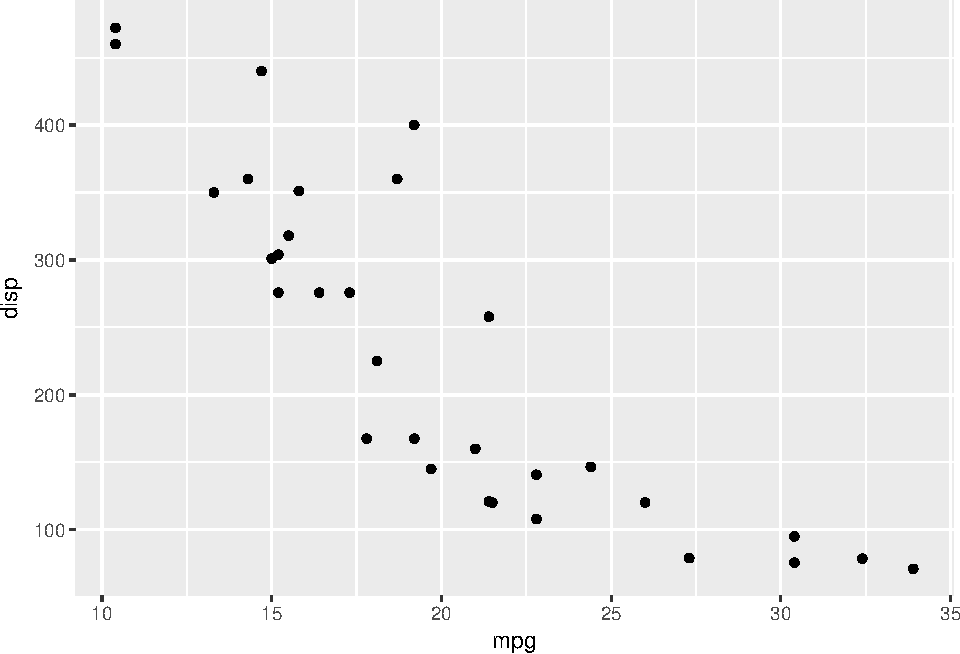
\includegraphics{visualization_files/figure-latex/unnamed-chunk-6-1.pdf}

It appears there is a negative relationship between miles per gallon and
engine size.

\section{Basic Exercise}\label{basic-exercise}

Now lets add another layer - a line - using the \texttt{geom\_line()}
function.

\section{Basic Exercise Solution}\label{basic-exercise-solution}

\begin{Shaded}
\begin{Highlighting}[]
\KeywordTok{ggplot}\NormalTok{(}\DataTypeTok{data =}\NormalTok{ cars, }\KeywordTok{aes}\NormalTok{(}\DataTypeTok{x =}\NormalTok{ mpg, }\DataTypeTok{y =}\NormalTok{ disp)) }\OperatorTok{+}
\StringTok{  }\KeywordTok{geom_point}\NormalTok{() }\OperatorTok{+}
\StringTok{  }\KeywordTok{geom_line}\NormalTok{()}
\end{Highlighting}
\end{Shaded}

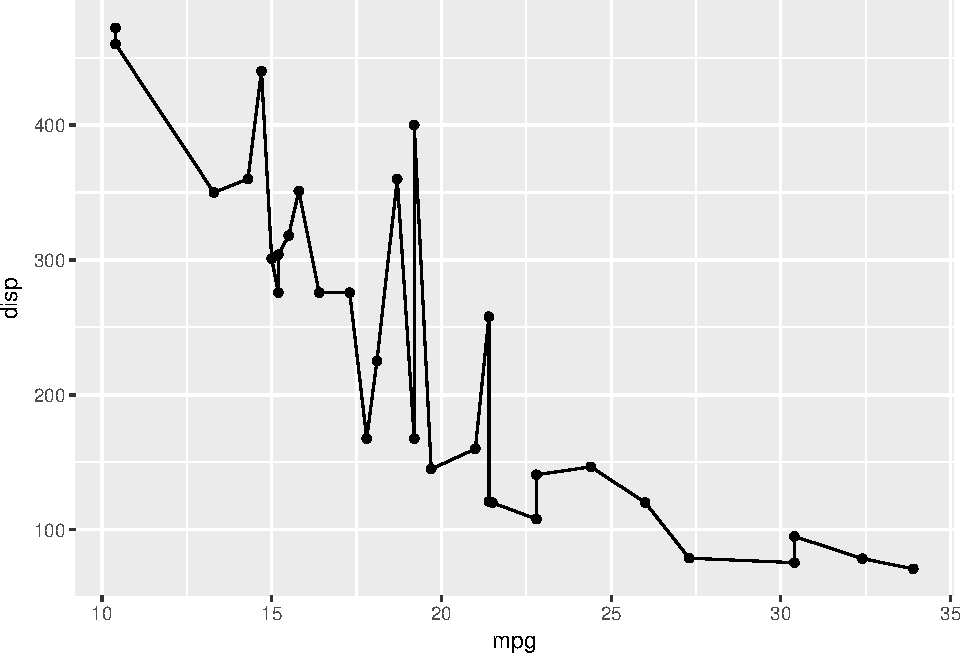
\includegraphics{visualization_files/figure-latex/unnamed-chunk-7-1.pdf}

\chapter{Customize}\label{customize}

There are nearly infinite possibilities for customizing charts with
\textbf{ggplot2}. We will focus on colors, labels, themes, and scales.

\section{Colors}\label{colors}

Using color is a great way to customize a visualization and make it more
interesting and easier to understand.

\begin{itemize}
\item
  R has over 600 colors built in which you can refer to by name.
\item
  The \texttt{colors()} function provides a list of the names.
\item
  You can also select colors by hexadecimal codes, such as ``\#990000''
  for deep red.
\item
  \href{http://www.cookbook-r.com/Graphs/Colors_(ggplot2)/}{R Cookbook
  Graphs section} has a very useful section on colors and palettes.
\item
  Another good reference for color palettes is
  \url{http://colorbrewer2.org}
\item
  The \emph{RColorBrewer} package provides a set of useful color
  palettes that can be used to customize the color ranges on a graph.
  Use \emph{display.brewer.all()} to see the set of palettes.
\item
  Note: Sometimes you will see the word ``color'' spelled ``colour'' -
  they are interchangeable in R.
\end{itemize}

Let's change the color of the points to purple, by setting it directly
in the \texttt{aes()} function of the geom.

\begin{Shaded}
\begin{Highlighting}[]
\KeywordTok{ggplot}\NormalTok{(}\DataTypeTok{data =}\NormalTok{ cars, }\KeywordTok{aes}\NormalTok{(}\DataTypeTok{x =}\NormalTok{ mpg, }\DataTypeTok{y =}\NormalTok{ disp)) }\OperatorTok{+}
\StringTok{  }\KeywordTok{geom_point}\NormalTok{(}\DataTypeTok{color =} \StringTok{"purple"}\NormalTok{)}
\end{Highlighting}
\end{Shaded}

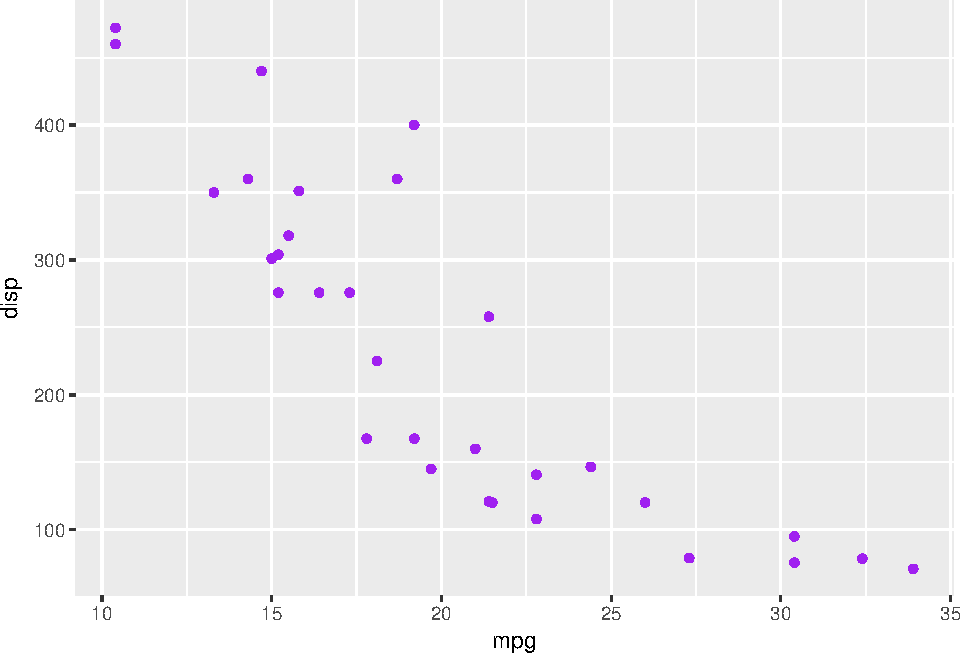
\includegraphics{visualization_files/figure-latex/unnamed-chunk-8-1.pdf}

You may also want to map the color of the points to another variable in
your dataset. This is done using the \texttt{aes()} function and setting
color equal to the variable name.

Let's map the color to the number of cylinders.

\begin{Shaded}
\begin{Highlighting}[]
\KeywordTok{ggplot}\NormalTok{(}\DataTypeTok{data =}\NormalTok{ cars, }\KeywordTok{aes}\NormalTok{(}\DataTypeTok{x =}\NormalTok{ mpg, }\DataTypeTok{y =}\NormalTok{ disp)) }\OperatorTok{+}
\StringTok{  }\KeywordTok{geom_point}\NormalTok{(}\KeywordTok{aes}\NormalTok{(}\DataTypeTok{color =}\NormalTok{ cyl))}
\end{Highlighting}
\end{Shaded}

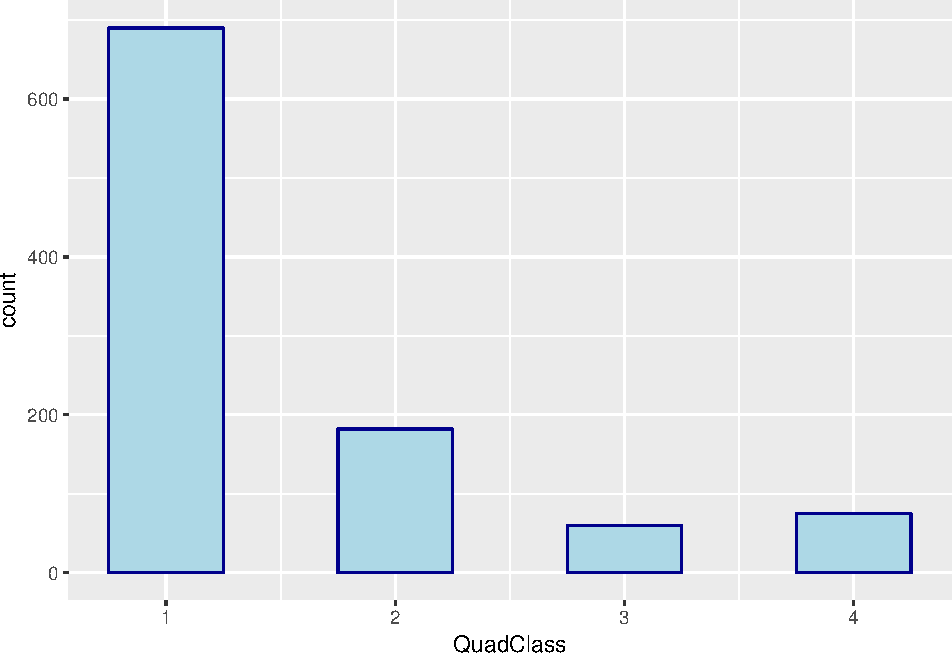
\includegraphics{visualization_files/figure-latex/unnamed-chunk-9-1.pdf}

Notice that a legend for the color is automatically added to the graph,
and a palette of blues is used by default. However, the cylinders
variable is treated as continuous but it is really just three values: 4,
6, and 8.

To treat the cylinders variable as categorical, you can convert it to a
factor inside the \texttt{ggplot()} function. Notice what happens to the
legend.

\begin{Shaded}
\begin{Highlighting}[]
\KeywordTok{ggplot}\NormalTok{(}\DataTypeTok{data =}\NormalTok{ cars, }\KeywordTok{aes}\NormalTok{(}\DataTypeTok{x =}\NormalTok{ mpg, }\DataTypeTok{y =}\NormalTok{ disp)) }\OperatorTok{+}
\StringTok{  }\KeywordTok{geom_point}\NormalTok{(}\KeywordTok{aes}\NormalTok{(}\DataTypeTok{color =} \KeywordTok{factor}\NormalTok{(cyl)))}
\end{Highlighting}
\end{Shaded}

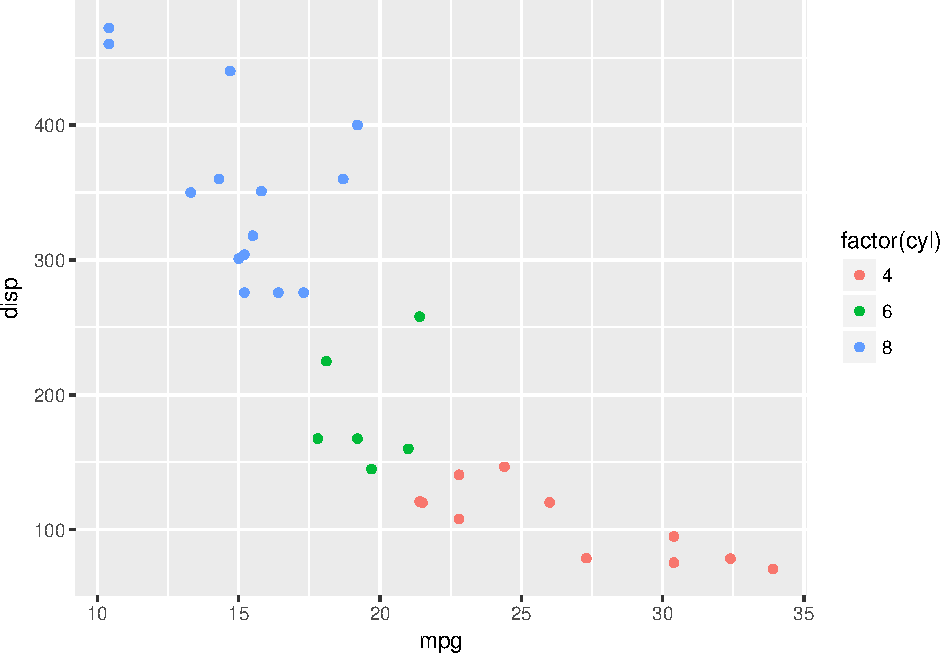
\includegraphics{visualization_files/figure-latex/unnamed-chunk-10-1.pdf}

\section{Labels}\label{labels}

You may want to customize the labels on the axes, using the
\texttt{xlab()} and \texttt{ylab()} functions. You can also add a graph
title to the \texttt{ggtitle()} function. Again, the ``+'' sign is used
to add these layers.

\begin{Shaded}
\begin{Highlighting}[]
\KeywordTok{ggplot}\NormalTok{(}\DataTypeTok{data =}\NormalTok{ cars, }\KeywordTok{aes}\NormalTok{(}\DataTypeTok{x =}\NormalTok{ mpg, }\DataTypeTok{y =}\NormalTok{ disp)) }\OperatorTok{+}
\StringTok{  }\KeywordTok{geom_point}\NormalTok{(}\KeywordTok{aes}\NormalTok{(}\DataTypeTok{color =} \KeywordTok{factor}\NormalTok{(cyl))) }\OperatorTok{+}
\StringTok{  }\KeywordTok{xlab}\NormalTok{(}\StringTok{"Miles Per Gallon"}\NormalTok{) }\OperatorTok{+}
\StringTok{  }\KeywordTok{ylab}\NormalTok{(}\StringTok{"Engine Size in Cubic Inches"}\NormalTok{) }\OperatorTok{+}
\StringTok{  }\KeywordTok{ggtitle}\NormalTok{(}\StringTok{"Fuel Efficiency vs Engine Size"}\NormalTok{)}
\end{Highlighting}
\end{Shaded}

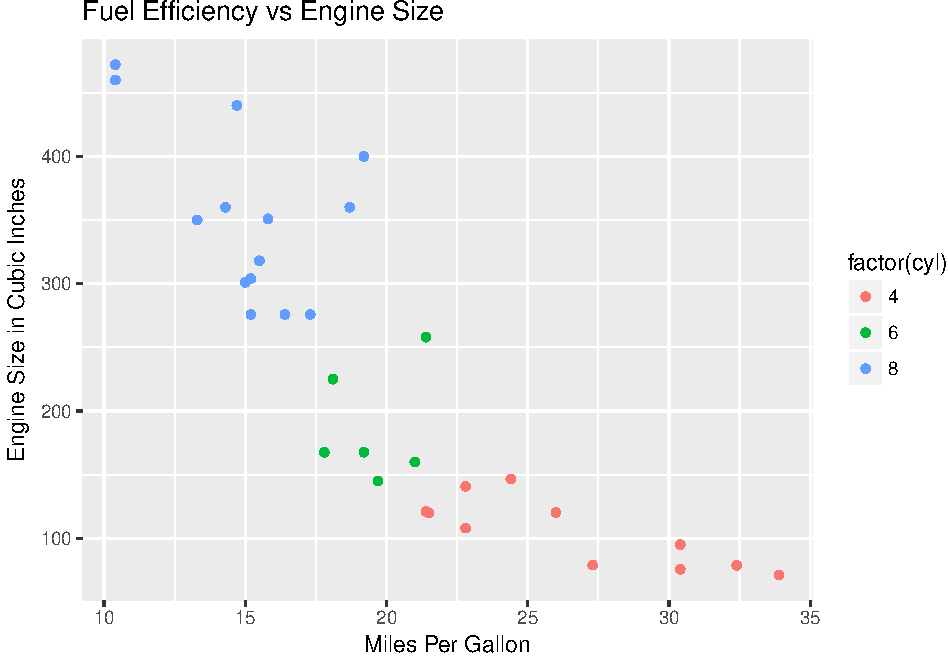
\includegraphics{visualization_files/figure-latex/unnamed-chunk-11-1.pdf}

\section{Customize Exercise}\label{customize-exercise}

Using the cars data:

\begin{enumerate}
\def\labelenumi{\arabic{enumi}.}
\item
  Plot wt versus hp with a scatterplot.
\item
  Color the points based on gear.
\item
  Change both axis labels - spell out wt and hp.
\item
  Add a chart title.
\end{enumerate}

\section{Customize Exercise Solution}\label{customize-exercise-solution}

\begin{Shaded}
\begin{Highlighting}[]
\KeywordTok{ggplot}\NormalTok{(}\DataTypeTok{data =}\NormalTok{ cars, }\KeywordTok{aes}\NormalTok{(}\DataTypeTok{x =}\NormalTok{ wt, }\DataTypeTok{y =}\NormalTok{ hp)) }\OperatorTok{+}
\StringTok{  }\KeywordTok{geom_point}\NormalTok{(}\KeywordTok{aes}\NormalTok{(}\DataTypeTok{color =} \KeywordTok{factor}\NormalTok{(gear))) }\OperatorTok{+}
\StringTok{  }\KeywordTok{xlab}\NormalTok{(}\StringTok{"Weight"}\NormalTok{) }\OperatorTok{+}
\StringTok{  }\KeywordTok{ylab}\NormalTok{(}\StringTok{"Horsepower"}\NormalTok{) }\OperatorTok{+}
\StringTok{  }\KeywordTok{ggtitle}\NormalTok{(}\StringTok{"How is power related to engine weight and number of gears?"}\NormalTok{)}
\end{Highlighting}
\end{Shaded}

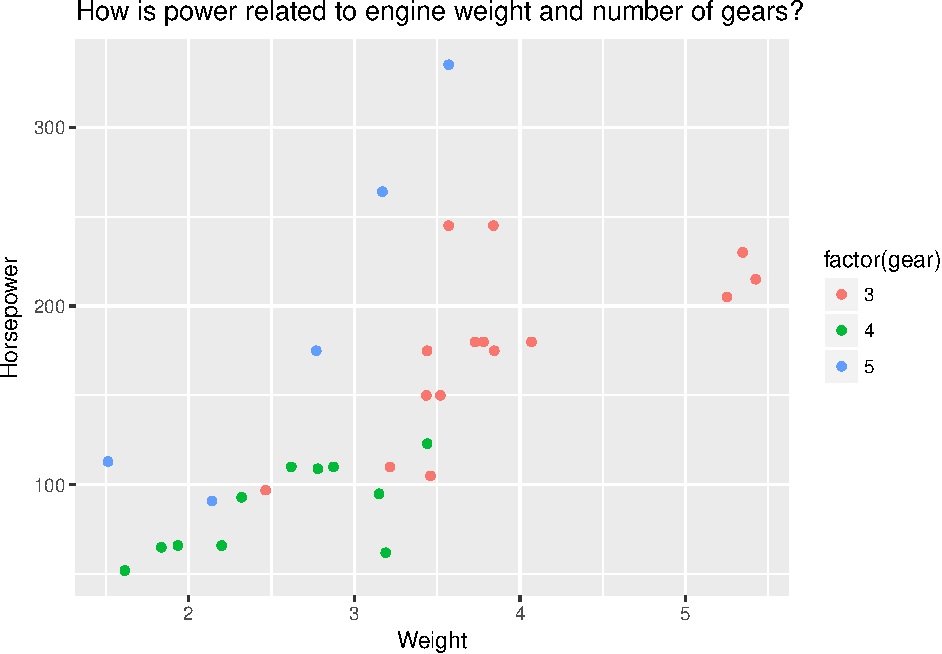
\includegraphics{visualization_files/figure-latex/unnamed-chunk-12-1.pdf}

\section{Themes}\label{themes}

There are many more options for customizing a graph. Adjusting the look
involves of two different types of elements, \emph{themes} and
\emph{scales}.

Theme elements are non-data components of the plot such as the title,
legend, and axes.

\begin{itemize}
\item
  To change the appearance of a theme element, use the \texttt{theme()}
  function on the component and identify the corresponding element
  object, such as ``element\_text''.
\item
  Common element objects are text or lines and not all element objects
  are associated with every component.
\item
  The
  \href{http://ase.tufts.edu/bugs/guide/assets/R\%20Graphics\%20Cookbook.pdf}{R
  Graphics Cookbook} covers this in section 9.4 very clearly.
\end{itemize}

Let's change the text of the axis labels:

\begin{itemize}
\item
  Font color of x-axis label to blue.
\item
  Font size of graph title to 20.
\end{itemize}

\begin{Shaded}
\begin{Highlighting}[]
\KeywordTok{ggplot}\NormalTok{(}\DataTypeTok{data =}\NormalTok{ cars, }\KeywordTok{aes}\NormalTok{(}\DataTypeTok{x =}\NormalTok{ mpg, }\DataTypeTok{y =}\NormalTok{ disp)) }\OperatorTok{+}
\StringTok{  }\KeywordTok{geom_point}\NormalTok{(}\KeywordTok{aes}\NormalTok{(}\DataTypeTok{color =} \KeywordTok{factor}\NormalTok{(cyl))) }\OperatorTok{+}
\StringTok{  }\KeywordTok{xlab}\NormalTok{(}\StringTok{"Miles Per Gallon"}\NormalTok{) }\OperatorTok{+}
\StringTok{  }\KeywordTok{ylab}\NormalTok{(}\StringTok{"Engine Size in Cubic Inches"}\NormalTok{) }\OperatorTok{+}
\StringTok{  }\KeywordTok{ggtitle}\NormalTok{(}\StringTok{"Fuel Efficiency vs Engine Size"}\NormalTok{) }\OperatorTok{+}
\StringTok{  }\KeywordTok{theme}\NormalTok{(}\DataTypeTok{axis.title.x =} \KeywordTok{element_text}\NormalTok{(}\DataTypeTok{color =} \StringTok{'blue'}\NormalTok{)) }\OperatorTok{+}
\StringTok{  }\KeywordTok{theme}\NormalTok{(}\DataTypeTok{plot.title =} \KeywordTok{element_text}\NormalTok{(}\DataTypeTok{size =} \DecValTok{20}\NormalTok{))}
\end{Highlighting}
\end{Shaded}

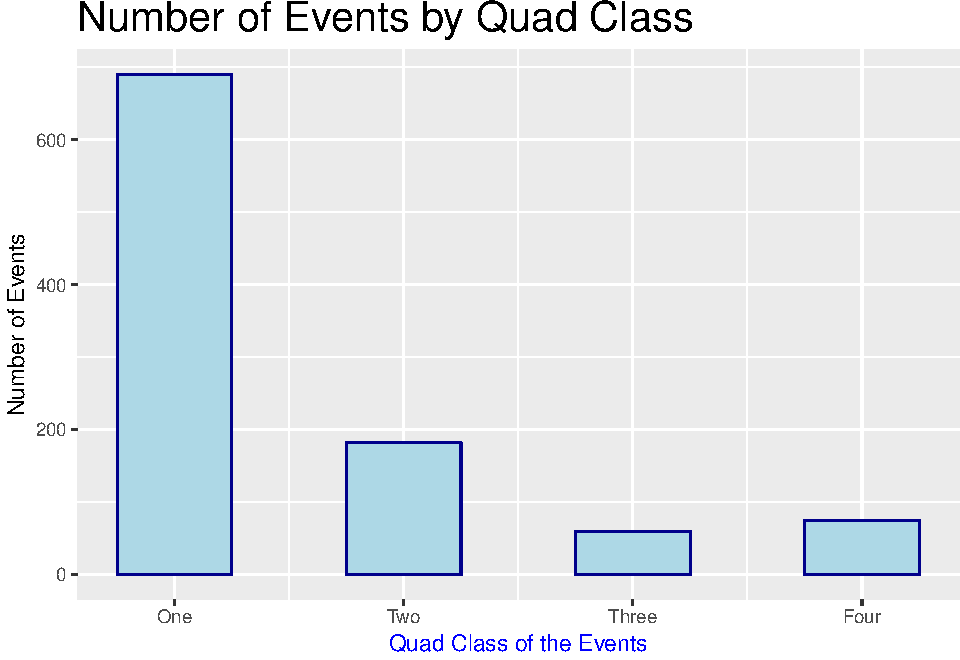
\includegraphics{visualization_files/figure-latex/unnamed-chunk-13-1.pdf}

A few other useful theme functions:

\begin{itemize}
\item
  Remove an axis label:
  \texttt{theme(axis.title.x\ =\ element\_blank())}
\item
  Remove grid lines:
  \texttt{theme(panel.grid.major\ =\ element\_blank())}
\item
  Rotate x-axis text labels by 90 degrees:
  \texttt{theme(axis.text.x\ =\ element\_text(angle\ =\ 90))}
\item
  Move the position of a legend:
  \texttt{theme(legend.position\ =\ "bottom")}
\end{itemize}

\section{Scales}\label{scales}

Scale elements map data values to visual values.

\begin{itemize}
\item
  To change the default mapping, a new scale layer is added.
\item
  A \texttt{scale} function identifies the aesthetic you want to adjust,
  a pre-packaged scale to use, and the specific arguments for what you
  are trying to change.
\item
  Different types of data use different types of aesthetics and scales -
  it is important to match them up correctly.
\item
  The \href{https://www.rstudio.com/resources/cheatsheets}{Data
  Visualization Cheatsheet} are a good reference for different types of
  scales.
\end{itemize}

We'll use \texttt{scale\_color\_manual()} and define the colors we want
use.

\begin{itemize}
\item
  ``scale'' indicates that we want to customize a data element.
\item
  ``color'' indicates which data element.
\item
  ``manual'' is used to specify the color mapping we want to use.
\end{itemize}

\begin{Shaded}
\begin{Highlighting}[]
\KeywordTok{ggplot}\NormalTok{(}\DataTypeTok{data =}\NormalTok{ cars, }\KeywordTok{aes}\NormalTok{(}\DataTypeTok{x =}\NormalTok{ mpg, }\DataTypeTok{y =}\NormalTok{ disp)) }\OperatorTok{+}
\StringTok{  }\KeywordTok{geom_point}\NormalTok{(}\KeywordTok{aes}\NormalTok{(}\DataTypeTok{color =} \KeywordTok{factor}\NormalTok{(cyl))) }\OperatorTok{+}
\StringTok{  }\KeywordTok{xlab}\NormalTok{(}\StringTok{"Miles Per Gallon"}\NormalTok{) }\OperatorTok{+}
\StringTok{  }\KeywordTok{ylab}\NormalTok{(}\StringTok{"Engine Size in Cubic Inches"}\NormalTok{) }\OperatorTok{+}
\StringTok{  }\KeywordTok{ggtitle}\NormalTok{(}\StringTok{"Fuel Efficiency vs Engine Size"}\NormalTok{) }\OperatorTok{+}
\StringTok{  }\KeywordTok{scale_color_manual}\NormalTok{(}\DataTypeTok{values =} \KeywordTok{c}\NormalTok{(}\StringTok{"red"}\NormalTok{,}\StringTok{"orange"}\NormalTok{,}\StringTok{"blue"}\NormalTok{))}
\end{Highlighting}
\end{Shaded}

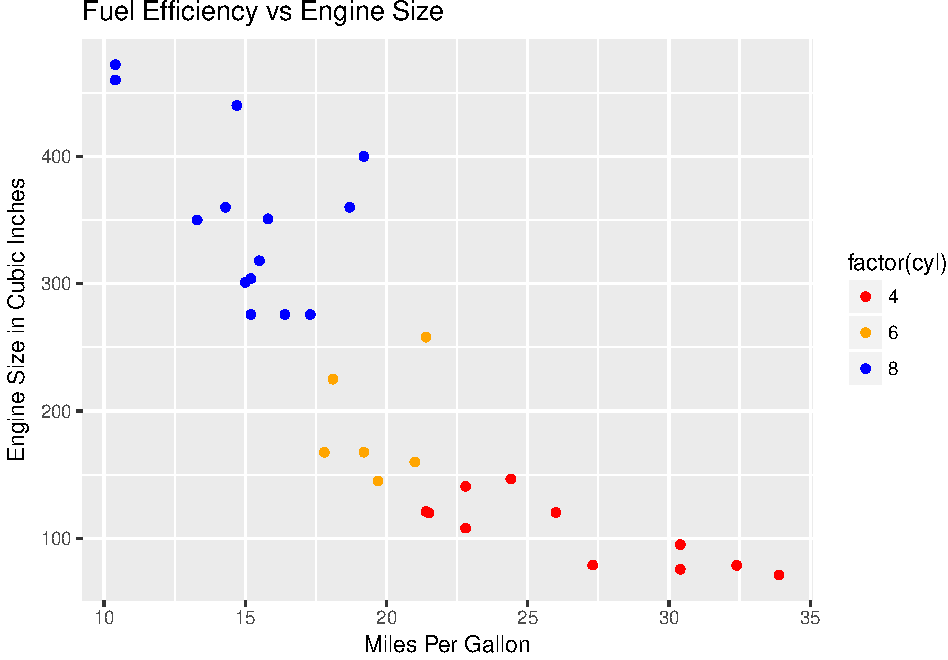
\includegraphics{visualization_files/figure-latex/unnamed-chunk-14-1.pdf}

\section{Single Scale Rule}\label{single-scale-rule}

Once you use a ``scale'' function on an aesthetic (in this case, color),
you need to include all the scale parameters in that function. If you
add another scale layer for the same aesthetic, it will replace the
previous layers.

Here's an example:

\begin{itemize}
\item
  Change the mapping for the color aesthetic from \emph{cyl} to the
  \emph{wt} variable, which is continuous.
\item
  You could use the \texttt{scale\_color\_continuous()} or
  \texttt{scale\_color\_gradient()} to effect the color aesthetic.
\item
  Let's change the color scheme with \texttt{scale\_color\_gradient()}
  and the breaks on the legend with \texttt{scale\_color\_continuous()}.
\end{itemize}

\begin{Shaded}
\begin{Highlighting}[]
\KeywordTok{ggplot}\NormalTok{(}\DataTypeTok{data =}\NormalTok{ cars, }\KeywordTok{aes}\NormalTok{(}\DataTypeTok{x =}\NormalTok{ mpg, }\DataTypeTok{y =}\NormalTok{ disp)) }\OperatorTok{+}
\StringTok{  }\KeywordTok{geom_point}\NormalTok{(}\KeywordTok{aes}\NormalTok{(}\DataTypeTok{color =}\NormalTok{ wt)) }\OperatorTok{+}
\StringTok{  }\KeywordTok{xlab}\NormalTok{(}\StringTok{"Miles Per Gallon"}\NormalTok{) }\OperatorTok{+}
\StringTok{  }\KeywordTok{ylab}\NormalTok{(}\StringTok{"Engine Size in Cubic Inches"}\NormalTok{) }\OperatorTok{+}
\StringTok{  }\KeywordTok{ggtitle}\NormalTok{(}\StringTok{"Fuel Efficiency vs Engine Size"}\NormalTok{) }\OperatorTok{+}
\StringTok{  }\KeywordTok{scale_color_gradient}\NormalTok{(}\DataTypeTok{low =} \StringTok{"red"}\NormalTok{, }\DataTypeTok{high =} \StringTok{"blue"}\NormalTok{) }\OperatorTok{+}
\StringTok{  }\KeywordTok{scale_color_continuous}\NormalTok{(}\DataTypeTok{breaks =} \KeywordTok{c}\NormalTok{(}\DecValTok{2}\NormalTok{,}\DecValTok{3}\NormalTok{,}\DecValTok{4}\NormalTok{,}\DecValTok{5}\NormalTok{))}
\end{Highlighting}
\end{Shaded}

\begin{verbatim}
## Scale for 'colour' is already present. Adding another scale for
## 'colour', which will replace the existing scale.
\end{verbatim}

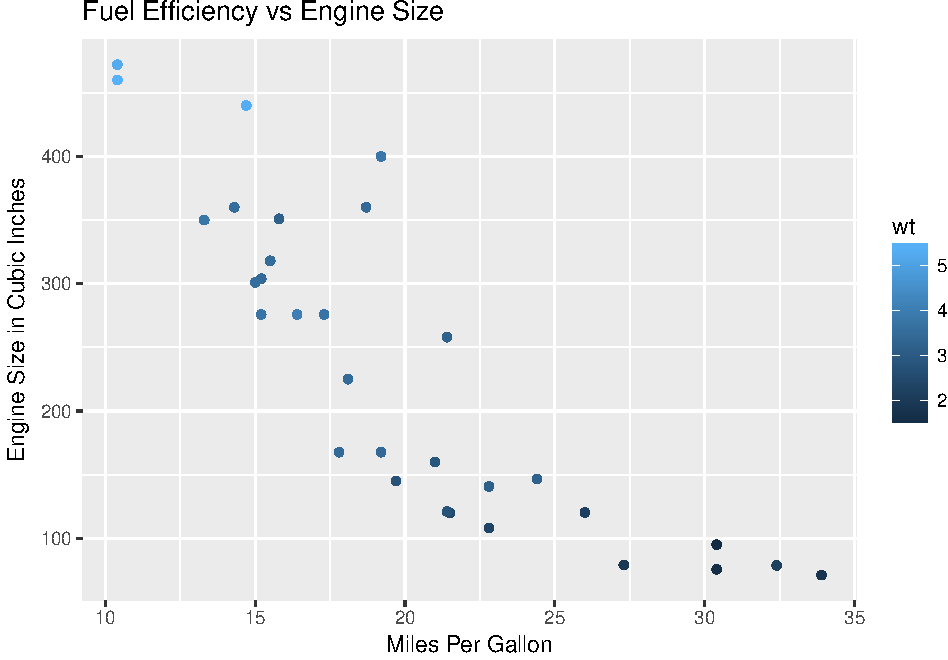
\includegraphics{visualization_files/figure-latex/unnamed-chunk-15-1.pdf}

But notice the error message and that the colors don't change.

Instead, combine the parameters into just one ``scale'' function.

\begin{Shaded}
\begin{Highlighting}[]
\KeywordTok{ggplot}\NormalTok{(}\DataTypeTok{data =}\NormalTok{ cars, }\KeywordTok{aes}\NormalTok{(}\DataTypeTok{x =}\NormalTok{ mpg, }\DataTypeTok{y =}\NormalTok{ disp)) }\OperatorTok{+}
\StringTok{  }\KeywordTok{geom_point}\NormalTok{(}\KeywordTok{aes}\NormalTok{(}\DataTypeTok{color =}\NormalTok{ wt)) }\OperatorTok{+}
\StringTok{  }\KeywordTok{xlab}\NormalTok{(}\StringTok{"Miles Per Gallon"}\NormalTok{) }\OperatorTok{+}
\StringTok{  }\KeywordTok{ylab}\NormalTok{(}\StringTok{"Engine Size in Cubic Inches"}\NormalTok{) }\OperatorTok{+}
\StringTok{  }\KeywordTok{ggtitle}\NormalTok{(}\StringTok{"Fuel Efficiency vs Engine Size"}\NormalTok{) }\OperatorTok{+}
\StringTok{  }\KeywordTok{scale_color_gradient}\NormalTok{(}\DataTypeTok{low =} \StringTok{"red"}\NormalTok{, }\DataTypeTok{high =} \StringTok{"blue"}\NormalTok{, }\DataTypeTok{breaks =} \KeywordTok{c}\NormalTok{(}\DecValTok{2}\NormalTok{,}\DecValTok{3}\NormalTok{,}\DecValTok{4}\NormalTok{,}\DecValTok{5}\NormalTok{)) }
\end{Highlighting}
\end{Shaded}

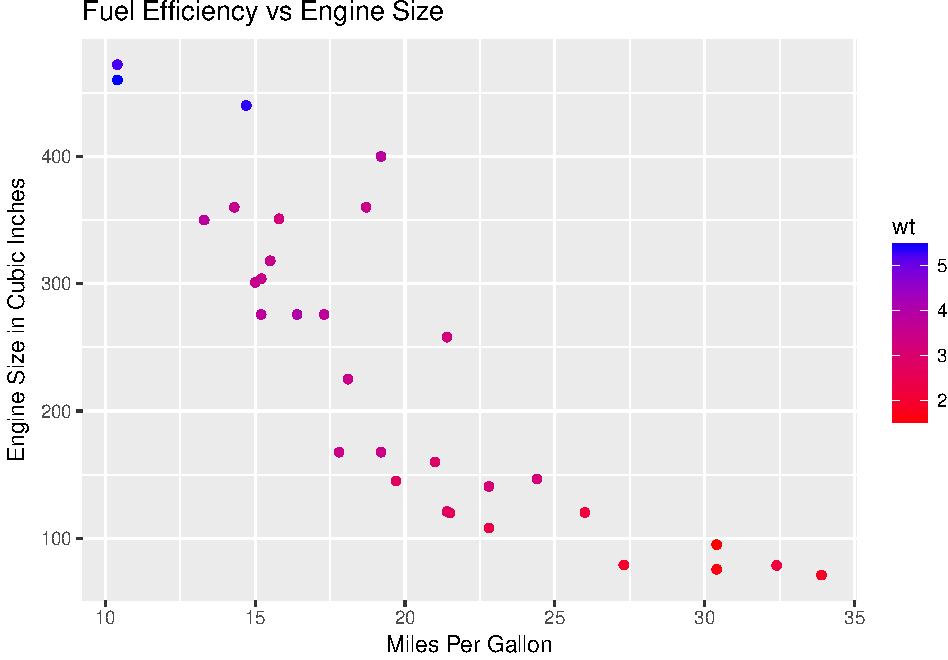
\includegraphics{visualization_files/figure-latex/unnamed-chunk-16-1.pdf}

\section{ggthemes}\label{ggthemes}

\textbf{ggthemes} is a package that provides some customized geoms,
scales, and themes.

\begin{itemize}
\tightlist
\item
  \url{https://github.com/jrnold/ggthemes}
\end{itemize}

\section{Saving Outputs}\label{saving-outputs}

To save your visualizations outside of RStudio, simply click the Export
button on the Plots tab.

Options:

\begin{itemize}
\item
  Save as an Image.
\item
  Save as a PDF.
\item
  Copy to Clipboard.
\end{itemize}

\chapter{Bar Charts}\label{bar-charts}

Bar charts are generally used to display numeric values on the y-axis
for different categories or discrete values on the x-axis. Bar charts
are not well suited for continuous data on the x-axis because it will
try to make a bar for every possible value of the continuous range.

\section{Thor Data}\label{thor-data}

For this section we will work with the THOR data from Vietnam, 1965.

\begin{Shaded}
\begin{Highlighting}[]
\NormalTok{nam65 <-}\StringTok{ }\KeywordTok{read.csv}\NormalTok{(}\StringTok{"thor_vietnam_65_clean.csv"}\NormalTok{, }\DataTypeTok{stringsAsFactors =} \OtherTok{FALSE}\NormalTok{)}
\KeywordTok{dim}\NormalTok{(nam65)}
\end{Highlighting}
\end{Shaded}

\begin{verbatim}
## [1] 63557    21
\end{verbatim}

This data set includes a subset of the variables from the raw THOR data
and cleaned up events with missing or inaccurate geospatial coordinates.

\section{geom\_bar}\label{geom_bar}

The heights of the bar on the y-axis can represent counts or values from
your data set. The code for the graph changes depending on which is the
case.

\begin{itemize}
\tightlist
\item
  The geom for bar charts is: \texttt{geom\_bar()}
\end{itemize}

Let's make a bar chart that shows the number of missions performed by
each military service.

\begin{itemize}
\tightlist
\item
  Use just one variable from our data set because we are interested in
  the counts for that variable.
\end{itemize}

\begin{Shaded}
\begin{Highlighting}[]
\KeywordTok{ggplot}\NormalTok{(}\DataTypeTok{data =}\NormalTok{ nam65, }\KeywordTok{aes}\NormalTok{(}\DataTypeTok{x =}\NormalTok{ MILSERVICE))}\OperatorTok{+}
\StringTok{  }\KeywordTok{geom_bar}\NormalTok{()}
\end{Highlighting}
\end{Shaded}

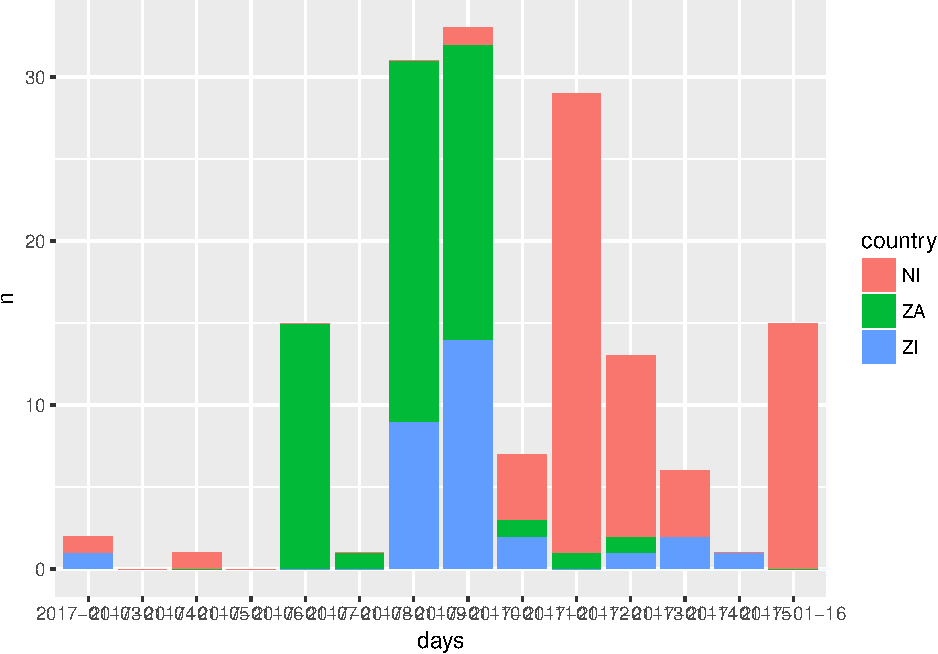
\includegraphics{visualization_files/figure-latex/unnamed-chunk-18-1.pdf}

Now we will add another variable called ``MFUNC\_DESC\_CLASS'', which
has two factor levels, ``KINETIC'' and ``NON-KINETIC''. We will use the
``fill'' aesthetic to map the new variable to the graph.

\begin{Shaded}
\begin{Highlighting}[]
\KeywordTok{ggplot}\NormalTok{(}\DataTypeTok{data =}\NormalTok{ nam65, }\KeywordTok{aes}\NormalTok{(}\DataTypeTok{x =}\NormalTok{ MILSERVICE, }\DataTypeTok{fill =}\NormalTok{ MFUNC_DESC_CLASS))}\OperatorTok{+}
\StringTok{  }\KeywordTok{geom_bar}\NormalTok{()}
\end{Highlighting}
\end{Shaded}

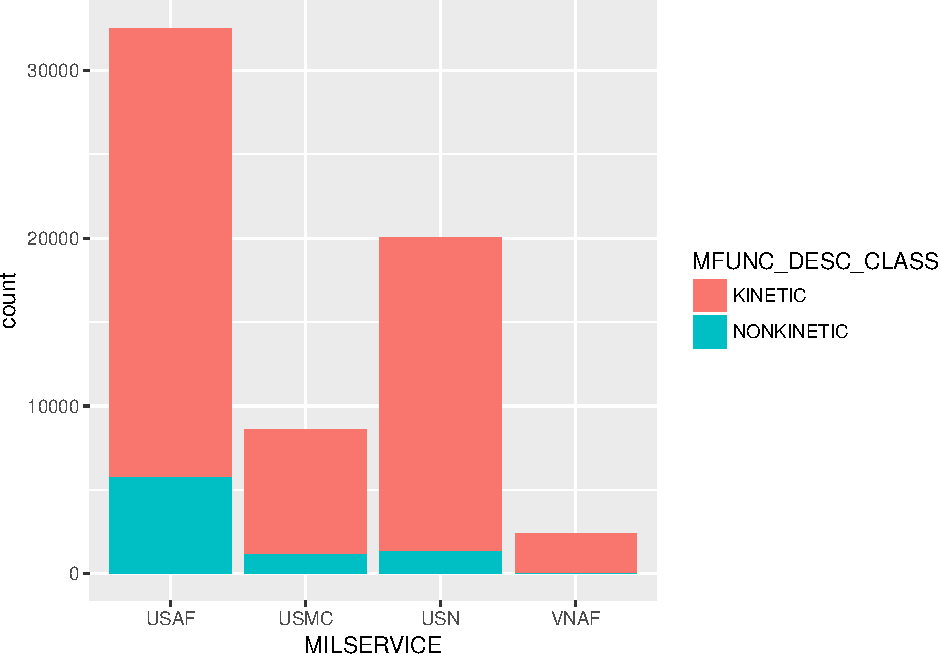
\includegraphics{visualization_files/figure-latex/unnamed-chunk-19-1.pdf}

Notice this creates a stacked bar. If you want to have bars side by side
for that variable, set the ``position'' parameter to ``dodge'' in the
geom like this: \texttt{geom\_bar(position\ =\ "dodge")}.

If we want to change the default colors, we use a ``scale'' function.

\begin{itemize}
\item
  Set the colors manually with:
  \texttt{scale\_fill\_manual(values\ =\ c("red","purple"))}
\item
  Use a palette from \emph{RColorBrewer} with:
  \texttt{scale\_fill\_brewer(palette\ =\ "Spectral")}
\end{itemize}

\section{Legends}\label{legends}

We want to make some changes to the legend on our chart.

\begin{itemize}
\item
  Change the legend title with \texttt{labs(fill\ =\ "Mission\ Type")}
\item
  Change the text of the labels with
  \texttt{scale\_fill\_discrete(labels\ =\ c("Kinetic","Non-Kinetic"))}
\end{itemize}

\begin{Shaded}
\begin{Highlighting}[]
\KeywordTok{ggplot}\NormalTok{(}\DataTypeTok{data =}\NormalTok{ nam65, }\KeywordTok{aes}\NormalTok{(}\DataTypeTok{x =}\NormalTok{ MILSERVICE, }\DataTypeTok{fill =}\NormalTok{ MFUNC_DESC_CLASS))}\OperatorTok{+}
\StringTok{  }\KeywordTok{geom_bar}\NormalTok{() }\OperatorTok{+}
\StringTok{  }\KeywordTok{labs}\NormalTok{(}\DataTypeTok{fill =} \StringTok{"Mission Type"}\NormalTok{) }\OperatorTok{+}
\StringTok{  }\KeywordTok{scale_fill_discrete}\NormalTok{(}\DataTypeTok{labels =} \KeywordTok{c}\NormalTok{(}\StringTok{"Kinetic"}\NormalTok{,}\StringTok{"Non-Kinetic"}\NormalTok{))}
\end{Highlighting}
\end{Shaded}

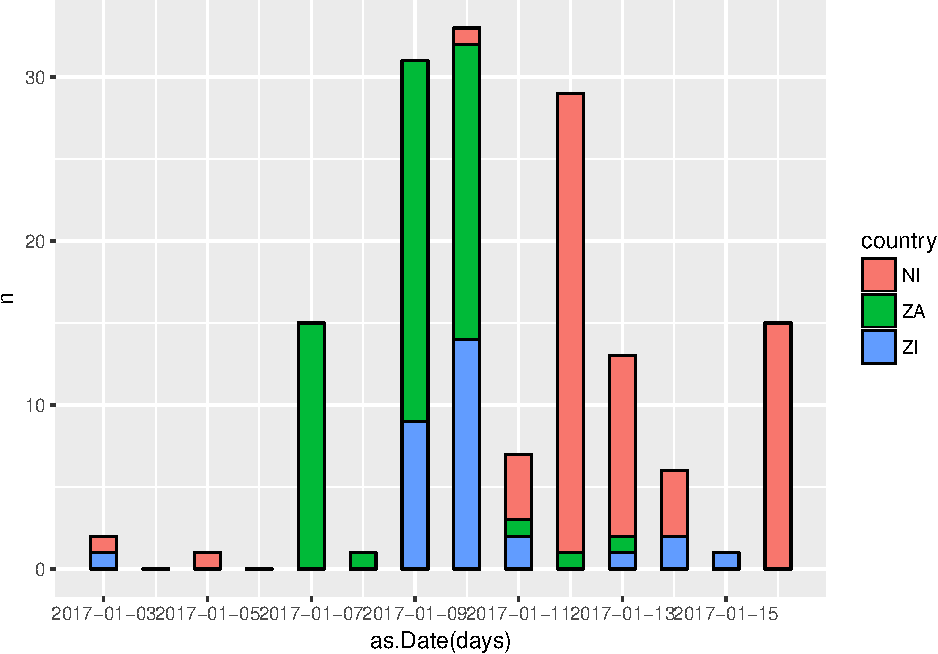
\includegraphics{visualization_files/figure-latex/unnamed-chunk-20-1.pdf}

\section{Bar Exercise}\label{bar-exercise}

Update our bar chart:

\begin{enumerate}
\def\labelenumi{\arabic{enumi}.}
\item
  Add a title
\item
  Remove the y-axis label (``count'')
\item
  Change the x-axis label
\item
  Change the colors for the fill aesthetic (don't forget the single
  scale rule!)
\end{enumerate}

\section{Bar Exercise Solution}\label{bar-exercise-solution}

\begin{Shaded}
\begin{Highlighting}[]
\KeywordTok{ggplot}\NormalTok{(}\DataTypeTok{data =}\NormalTok{ nam65, }\KeywordTok{aes}\NormalTok{(}\DataTypeTok{x =}\NormalTok{ MILSERVICE, }\DataTypeTok{fill =}\NormalTok{ MFUNC_DESC_CLASS))}\OperatorTok{+}
\StringTok{  }\KeywordTok{geom_bar}\NormalTok{() }\OperatorTok{+}
\StringTok{  }\KeywordTok{labs}\NormalTok{(}\DataTypeTok{fill =} \StringTok{"Mission Type"}\NormalTok{) }\OperatorTok{+}
\StringTok{  }\CommentTok{#scale_fill_discrete(labels = c("Kinetic","Non-Kinetic")) +      #single scale rule!}
\StringTok{  }\KeywordTok{ggtitle}\NormalTok{(}\StringTok{"Missions by Each Service"}\NormalTok{) }\OperatorTok{+}
\StringTok{  }\KeywordTok{theme}\NormalTok{(}\DataTypeTok{axis.title.y =} \KeywordTok{element_blank}\NormalTok{()) }\OperatorTok{+}
\StringTok{  }\KeywordTok{xlab}\NormalTok{(}\StringTok{"Military Service"}\NormalTok{) }\OperatorTok{+}
\StringTok{  }\KeywordTok{scale_fill_brewer}\NormalTok{(}\DataTypeTok{palette =} \StringTok{"Dark2"}\NormalTok{,}\DataTypeTok{labels =} \KeywordTok{c}\NormalTok{(}\StringTok{"Kinetic"}\NormalTok{,}\StringTok{"Non-Kinetic"}\NormalTok{))   }\CommentTok{#single scale rule!}
\end{Highlighting}
\end{Shaded}

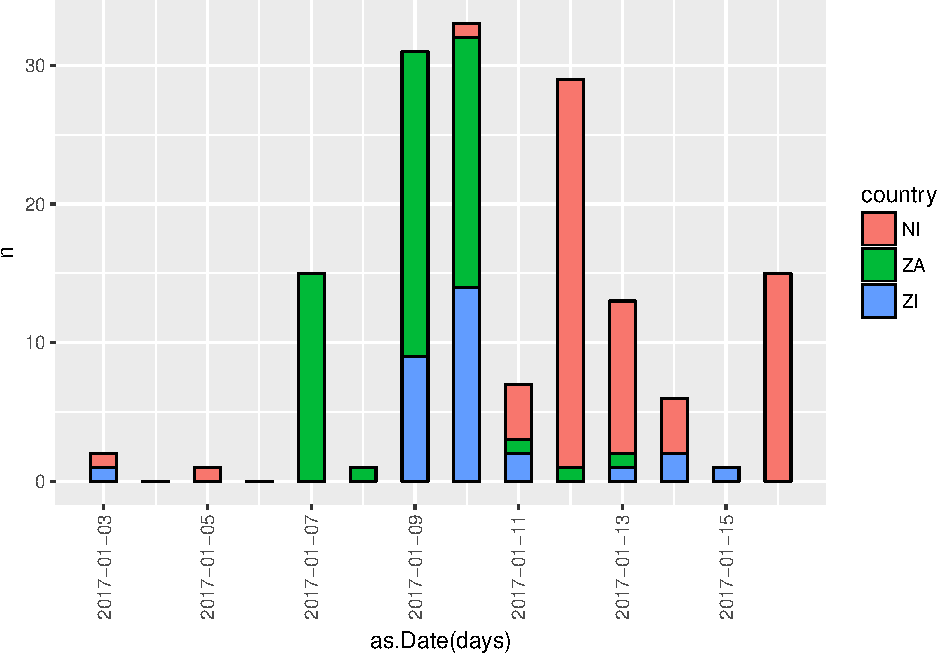
\includegraphics{visualization_files/figure-latex/unnamed-chunk-21-1.pdf}

\chapter{Barcharts with Values}\label{barcharts-with-values}

Remember that there's a difference in how to make a bar chart with
values from a variable in the data on the y-axis vice counts for a
single variable.

\section{Aircraft Data}\label{aircraft-data}

For this example, we will summarize the average number of aircraft per
mission across the different target types.

\begin{Shaded}
\begin{Highlighting}[]
\NormalTok{aircraft <-}\StringTok{ }\KeywordTok{summarize}\NormalTok{(}\KeywordTok{group_by}\NormalTok{(nam65, TGTTYPE), }\DataTypeTok{avgNumAcft =} \KeywordTok{mean}\NormalTok{(NUMOFACFT))}
\KeywordTok{head}\NormalTok{(aircraft)}
\end{Highlighting}
\end{Shaded}

\begin{verbatim}
## # A tibble: 6 x 2
##              TGTTYPE avgNumAcft
##                <chr>      <dbl>
## 1                      3.163743
## 2 AIRCRAFT (UNIDENT)   2.400000
## 3           AIRFIELD   1.742788
## 4      ANTI-AIRCRAFT   2.504082
## 5      "AREA\\DEPOT"   2.811982
## 6             BRIDGE   2.559007
\end{verbatim}

Notice that the first row is missing the target type information. Let's
fill in the blank space.

\begin{Shaded}
\begin{Highlighting}[]
\NormalTok{aircraft[}\DecValTok{1}\NormalTok{,}\DecValTok{1}\NormalTok{] <-}\StringTok{ "UNIDENTIFIED"}
\KeywordTok{head}\NormalTok{(aircraft)}
\end{Highlighting}
\end{Shaded}

\begin{verbatim}
## # A tibble: 6 x 2
##              TGTTYPE avgNumAcft
##                <chr>      <dbl>
## 1       UNIDENTIFIED   3.163743
## 2 AIRCRAFT (UNIDENT)   2.400000
## 3           AIRFIELD   1.742788
## 4      ANTI-AIRCRAFT   2.504082
## 5      "AREA\\DEPOT"   2.811982
## 6             BRIDGE   2.559007
\end{verbatim}

\section{Stat Parameter}\label{stat-parameter}

To make a barchart of this data, you need to set the ``stat'' parameter
in the \texttt{geom\_bar()} function to ``identity'', instead of the
default ``bin''.

\begin{itemize}
\item
  The ``stat'' refers to the statistical transformation that ggplot does
  on the raw data, which by default in bar charts is set to bin and
  count the number of points for each bin.
\item
  To use the variable data on the y-axis instead of the count, you need
  to change the ``stat'' parameter.
\end{itemize}

For this example, we want to see the average number of aircraft (y-axis)
per target type (x-axis).

\begin{Shaded}
\begin{Highlighting}[]
\KeywordTok{ggplot}\NormalTok{(}\DataTypeTok{data =}\NormalTok{ aircraft, }\KeywordTok{aes}\NormalTok{(}\DataTypeTok{x =}\NormalTok{ TGTTYPE, }\DataTypeTok{y =}\NormalTok{ avgNumAcft))}\OperatorTok{+}
\StringTok{  }\KeywordTok{geom_bar}\NormalTok{(}\DataTypeTok{stat=} \StringTok{"identity"}\NormalTok{)}
\end{Highlighting}
\end{Shaded}

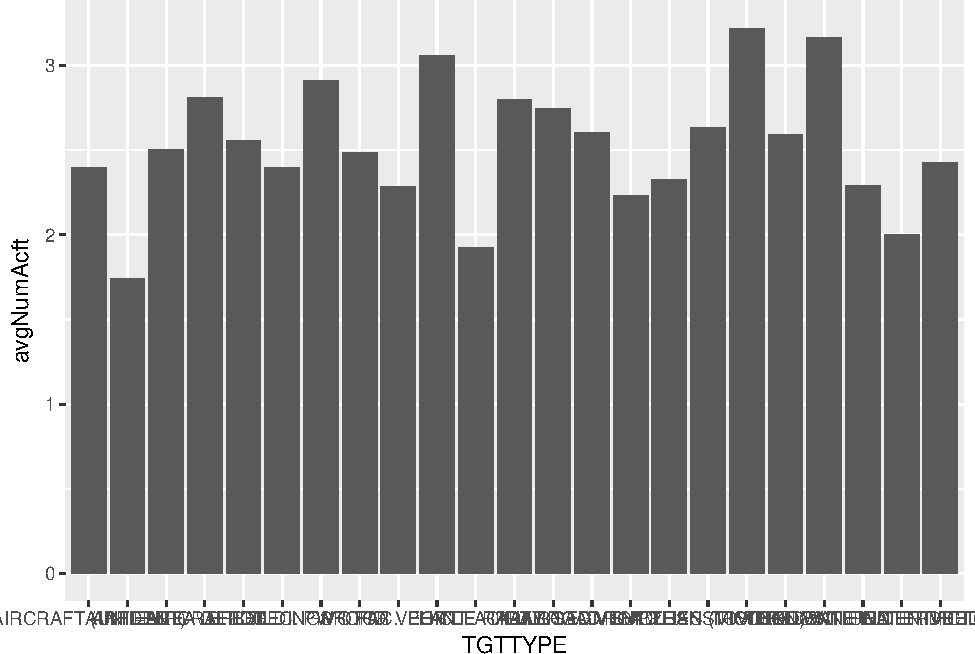
\includegraphics{visualization_files/figure-latex/unnamed-chunk-24-1.pdf}

\section{hjust and vjust}\label{hjust-and-vjust}

The ``hjust'' and ``vjust'' parameters in the \texttt{theme()} function
for an axis change the horizontal and vertical justification of the
text.

\begin{itemize}
\item
  These work in conjunction with the ``angle'' parameter to make the
  text more readable.
\item
  A good reference for this is
  \url{https://www.r-bloggers.com/hjust-and-vjust/}
\item
  Note that each parameter can only take certain values and the
  combination results in different positions.
\item
  The theme function looks like:
  \texttt{theme(axis.text.x\ =\ element\_text(angle\ =\ 90,\ hjust\ =\ 1,\ vjust\ =\ .5))}
\end{itemize}

\section{Sorting Bars}\label{sorting-bars}

We can sort the bars by height using the \texttt{reorder()} function in
the \texttt{aes()} for the x-axis.

\begin{Shaded}
\begin{Highlighting}[]
\KeywordTok{ggplot}\NormalTok{(}\DataTypeTok{data =}\NormalTok{ aircraft, }\KeywordTok{aes}\NormalTok{(}\DataTypeTok{x =} \KeywordTok{reorder}\NormalTok{(TGTTYPE, avgNumAcft), }\DataTypeTok{y =}\NormalTok{ avgNumAcft))}\OperatorTok{+}
\StringTok{  }\KeywordTok{geom_bar}\NormalTok{(}\DataTypeTok{stat=} \StringTok{"identity"}\NormalTok{, }\DataTypeTok{fill =} \StringTok{"blue"}\NormalTok{) }\OperatorTok{+}
\StringTok{  }\KeywordTok{theme}\NormalTok{(}\DataTypeTok{axis.text.x =} \KeywordTok{element_text}\NormalTok{(}\DataTypeTok{angle =} \DecValTok{90}\NormalTok{, }\DataTypeTok{hjust =} \DecValTok{1}\NormalTok{, }\DataTypeTok{vjust =}\NormalTok{ .}\DecValTok{5}\NormalTok{)) }\OperatorTok{+}
\StringTok{  }\KeywordTok{ggtitle}\NormalTok{(}\StringTok{"Do Different Types of Targets Involve More Aircraft?"}\NormalTok{) }\OperatorTok{+}
\StringTok{  }\KeywordTok{theme}\NormalTok{(}\DataTypeTok{plot.title =} \KeywordTok{element_text}\NormalTok{(}\DataTypeTok{size =} \DecValTok{14}\NormalTok{)) }\OperatorTok{+}
\StringTok{  }\KeywordTok{xlab}\NormalTok{(}\StringTok{"Target Type"}\NormalTok{) }\OperatorTok{+}
\StringTok{  }\KeywordTok{ylab}\NormalTok{(}\StringTok{"Average Number of Aircraft"}\NormalTok{)}
\end{Highlighting}
\end{Shaded}

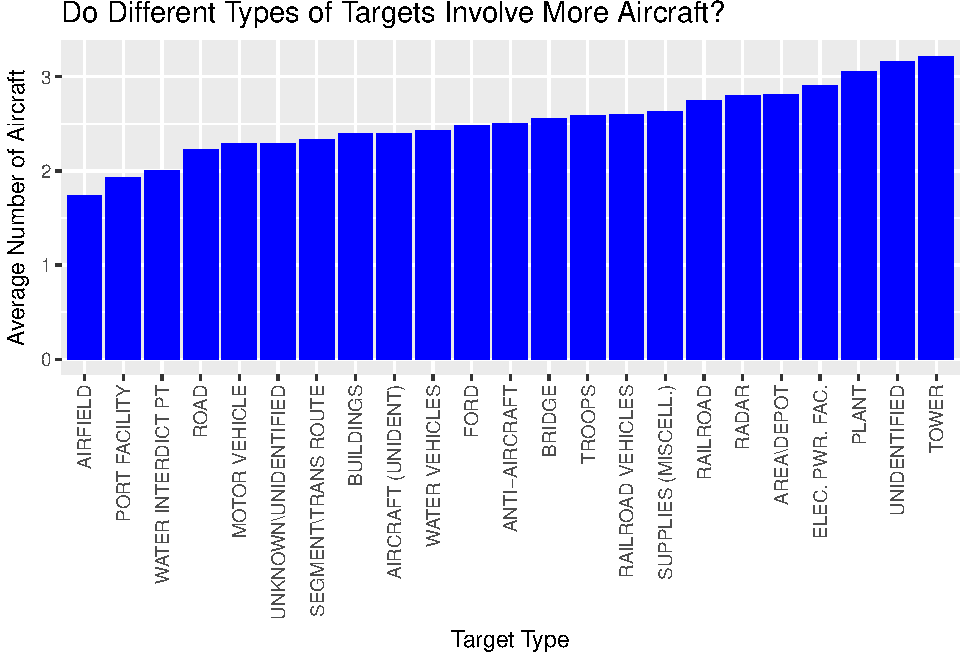
\includegraphics{visualization_files/figure-latex/unnamed-chunk-25-1.pdf}

You can also change the sort to from most to least like this:
\texttt{aes(x\ =\ reorder(TGTTYPE,\ desc(avgNumAcft)),\ y\ =\ avgNumAcft)}

\section{Bar with Values Exercise}\label{bar-with-values-exercise}

Update the average number of aircraft per target type chart with:

\begin{enumerate}
\def\labelenumi{\arabic{enumi}.}
\item
  Create a dataframe with the number of missions per mission type (hint:
  MFUNC\_DESC variable)
\item
  Make a bar chart that displays the 20 most frequent mission types, in
  descending order.
\item
  Rotate the labels on the x-axis to make it readable.
\item
  Add a chart title and make it a larger font.
\item
  Change the axis titles.
\item
  Change the color of the bars to blue.
\end{enumerate}

\section{Bar with Values Exercise
Solution}\label{bar-with-values-exercise-solution}

\begin{Shaded}
\begin{Highlighting}[]
\NormalTok{bar_y <-}\StringTok{ }\KeywordTok{summarize}\NormalTok{(}\KeywordTok{group_by}\NormalTok{(nam65, MFUNC_DESC), }\DataTypeTok{num_missions =} \KeywordTok{n}\NormalTok{())}
\NormalTok{bar_y <-}\StringTok{ }\KeywordTok{arrange}\NormalTok{(bar_y, }\KeywordTok{desc}\NormalTok{(num_missions))}
\NormalTok{bar_y <-}\StringTok{ }\NormalTok{bar_y[}\DecValTok{1}\OperatorTok{:}\DecValTok{20}\NormalTok{,]}

\KeywordTok{ggplot}\NormalTok{(}\DataTypeTok{data =}\NormalTok{ bar_y, }\KeywordTok{aes}\NormalTok{(}\DataTypeTok{x =} \KeywordTok{reorder}\NormalTok{(MFUNC_DESC, }\KeywordTok{desc}\NormalTok{(num_missions)), }\DataTypeTok{y =}\NormalTok{ num_missions))}\OperatorTok{+}
\StringTok{  }\KeywordTok{geom_bar}\NormalTok{(}\DataTypeTok{stat =} \StringTok{"identity"}\NormalTok{, }\DataTypeTok{fill =} \StringTok{"blue"}\NormalTok{)}\OperatorTok{+}
\StringTok{  }\KeywordTok{theme}\NormalTok{(}\DataTypeTok{axis.text.x =} \KeywordTok{element_text}\NormalTok{(}\DataTypeTok{angle =} \DecValTok{90}\NormalTok{, }\DataTypeTok{hjust =} \DecValTok{1}\NormalTok{, }\DataTypeTok{vjust =}\NormalTok{ .}\DecValTok{5}\NormalTok{)) }\OperatorTok{+}
\StringTok{  }\KeywordTok{ggtitle}\NormalTok{(}\StringTok{"Most Frequent Mission Types"}\NormalTok{) }\OperatorTok{+}
\StringTok{  }\KeywordTok{theme}\NormalTok{(}\DataTypeTok{plot.title =} \KeywordTok{element_text}\NormalTok{(}\DataTypeTok{size =} \DecValTok{14}\NormalTok{)) }\OperatorTok{+}
\StringTok{  }\KeywordTok{xlab}\NormalTok{(}\StringTok{"Mission Type"}\NormalTok{) }\OperatorTok{+}
\StringTok{  }\KeywordTok{ylab}\NormalTok{(}\StringTok{"Number of Missions"}\NormalTok{)}
\end{Highlighting}
\end{Shaded}

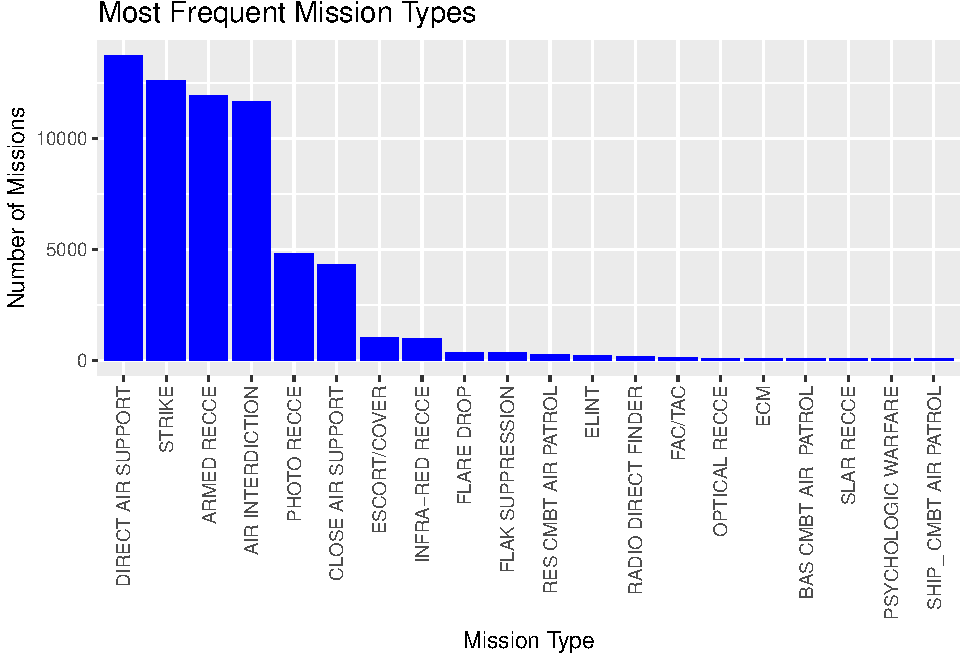
\includegraphics{visualization_files/figure-latex/unnamed-chunk-26-1.pdf}

\chapter{Line Charts}\label{line-charts}

A time series is a series of data points indexed in time order, most
commonly in an equally spaced sequence. While this makes the data
discrete, you often see a time series visualized with a line. We will
create our line charts once again with the \textbf{ggplot2} package.

\section{Missions Per Day}\label{missions-per-day}

Let's make a time series chart of the missions, showing the number of
missions each day.

First we need to format the ``MSNDATE'' variable using the
\textbf{lubridate} package. This will fix the inconsistent date formats.

\begin{Shaded}
\begin{Highlighting}[]
\NormalTok{nam65}\OperatorTok{$}\NormalTok{MSNDATE<-lubridate}\OperatorTok{::}\KeywordTok{ymd}\NormalTok{(nam65}\OperatorTok{$}\NormalTok{MSNDATE)}
\end{Highlighting}
\end{Shaded}

Notice that the data type for ``MSNDATE'' changed to Date.

Next, we need to count the number of missions per day.

\begin{Shaded}
\begin{Highlighting}[]
\NormalTok{msn <-}\StringTok{ }\KeywordTok{summarise}\NormalTok{(}\KeywordTok{group_by}\NormalTok{(nam65, MSNDATE), }\DataTypeTok{missions =} \KeywordTok{n}\NormalTok{())}
\KeywordTok{dim}\NormalTok{(msn)}
\end{Highlighting}
\end{Shaded}

\begin{verbatim}
## [1] 92  2
\end{verbatim}

Notice that there are 92 days from 1Oct65 to 31Dec65, and there are 92
rows in our new dataframe, indicating that there are no missing dates.

To do time series, you need to make sure there are no missing dates. You
may need to fill in the data set with zeros for dates that are missing
or aggregate to a lower level of precision.

\section{geom\_line}\label{geom_line}

Now we will create our plot, using \texttt{geom\_line()}.

\begin{Shaded}
\begin{Highlighting}[]
\KeywordTok{ggplot}\NormalTok{(msn, }\KeywordTok{aes}\NormalTok{(}\DataTypeTok{x =}\NormalTok{ MSNDATE, }\DataTypeTok{y =}\NormalTok{ missions))}\OperatorTok{+}
\StringTok{  }\KeywordTok{geom_line}\NormalTok{()}
\end{Highlighting}
\end{Shaded}

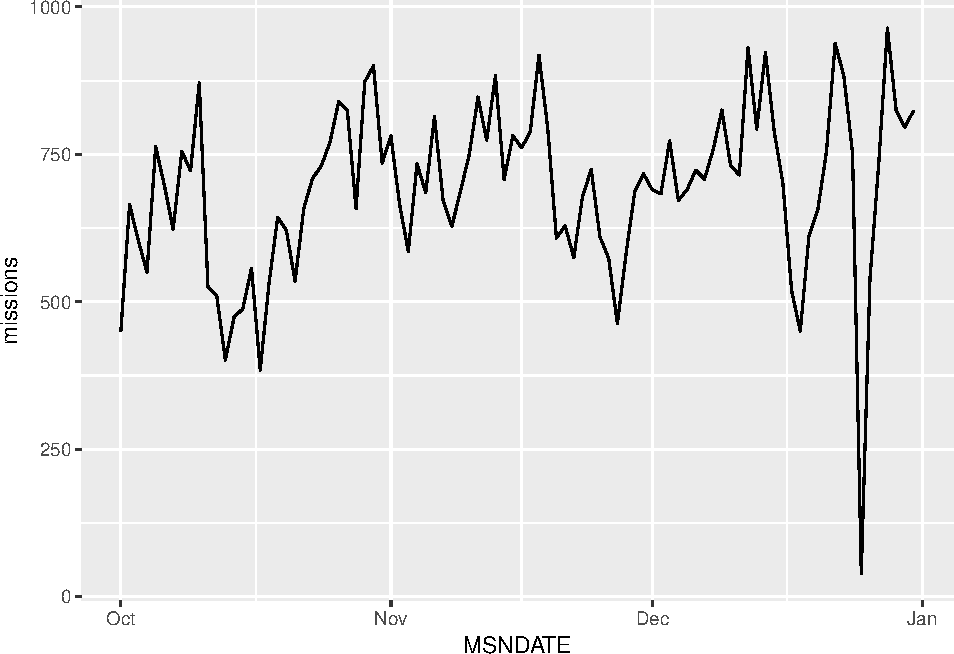
\includegraphics{visualization_files/figure-latex/unnamed-chunk-29-1.pdf}

\section{Date Scales}\label{date-scales}

Notice that ggplot only used the months as labels on the x-axis. To
create weekly breaks across the time series, use the \texttt{seq()} and
\texttt{as.Date()} functions.

\begin{Shaded}
\begin{Highlighting}[]
\NormalTok{datebreaks<-}\KeywordTok{seq}\NormalTok{(}\KeywordTok{as.Date}\NormalTok{(}\StringTok{"1965-10-01"}\NormalTok{),}\KeywordTok{as.Date}\NormalTok{(}\StringTok{"1965-12-31"}\NormalTok{), }\DataTypeTok{by=}\StringTok{"week"}\NormalTok{)}
\KeywordTok{head}\NormalTok{(datebreaks)}
\end{Highlighting}
\end{Shaded}

\begin{verbatim}
## [1] "1965-10-01" "1965-10-08" "1965-10-15" "1965-10-22" "1965-10-29"
## [6] "1965-11-05"
\end{verbatim}

To change the labels on the x-axis:

\begin{itemize}
\item
  Use a \texttt{scale\_x\_date()} function to adjust the labels on the
  x-axis with the ``datebreaks'' vector.
\item
  Use the \texttt{date\_format()} function from the \textbf{scales}
  package to change the format of the dates to ``day-month-year''.
\end{itemize}

\begin{Shaded}
\begin{Highlighting}[]
\KeywordTok{ggplot}\NormalTok{(msn,}\KeywordTok{aes}\NormalTok{(}\DataTypeTok{x=}\NormalTok{MSNDATE, }\DataTypeTok{y=}\NormalTok{ missions))}\OperatorTok{+}
\StringTok{  }\KeywordTok{geom_line}\NormalTok{()}\OperatorTok{+}
\StringTok{  }\KeywordTok{scale_x_date}\NormalTok{(}\DataTypeTok{breaks=}\NormalTok{datebreaks, }\DataTypeTok{labels =} \KeywordTok{date_format}\NormalTok{(}\StringTok{"%d-%b-%y"}\NormalTok{)) }\OperatorTok{+}
\StringTok{  }\KeywordTok{theme}\NormalTok{(}\DataTypeTok{axis.text.x=}\KeywordTok{element_text}\NormalTok{(}\DataTypeTok{angle=}\DecValTok{90}\NormalTok{, }\DataTypeTok{hjust=}\DecValTok{1}\NormalTok{, }\DataTypeTok{vjust =}\NormalTok{ .}\DecValTok{5}\NormalTok{)) }
\end{Highlighting}
\end{Shaded}

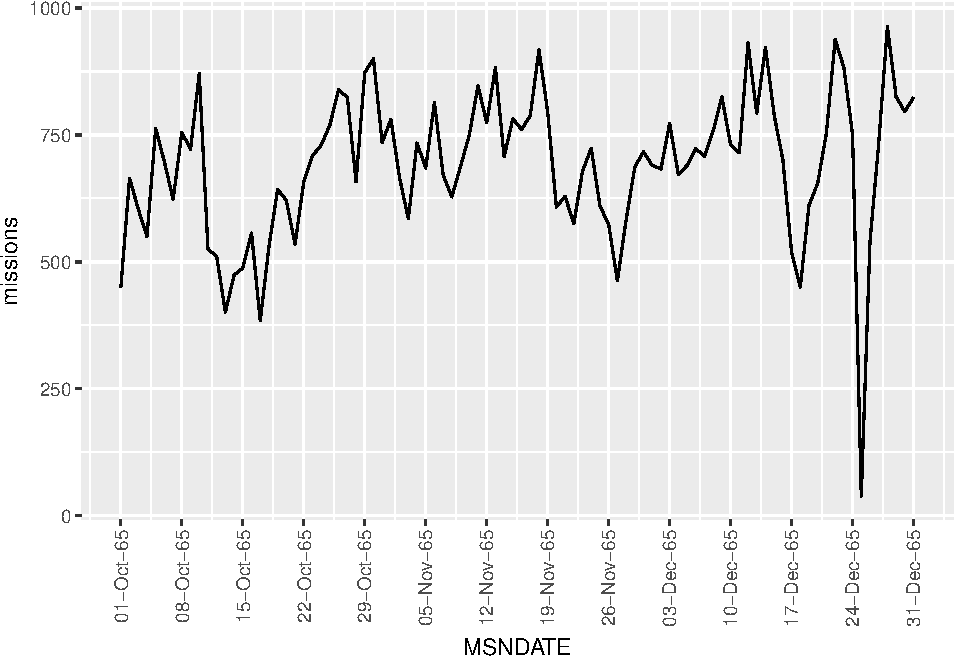
\includegraphics{visualization_files/figure-latex/unnamed-chunk-31-1.pdf}

\section{Annotation}\label{annotation}

The deep dip in our time series chart occurs on Christmas Day. (hint:
use the \texttt{arrange()} function to determine that) We can label that
information on the chart using the \texttt{annotate()} function in the
ggplot.

\begin{Shaded}
\begin{Highlighting}[]
\KeywordTok{ggplot}\NormalTok{(msn,}\KeywordTok{aes}\NormalTok{(}\DataTypeTok{x=}\NormalTok{MSNDATE, }\DataTypeTok{y=}\NormalTok{ missions))}\OperatorTok{+}
\StringTok{  }\KeywordTok{geom_line}\NormalTok{()}\OperatorTok{+}
\StringTok{  }\KeywordTok{scale_x_date}\NormalTok{(}\DataTypeTok{breaks=}\NormalTok{datebreaks, }\DataTypeTok{labels =} \KeywordTok{date_format}\NormalTok{(}\StringTok{"%d-%b-%y"}\NormalTok{)) }\OperatorTok{+}
\StringTok{  }\KeywordTok{theme}\NormalTok{(}\DataTypeTok{axis.text.x=}\KeywordTok{element_text}\NormalTok{(}\DataTypeTok{angle=}\DecValTok{90}\NormalTok{, }\DataTypeTok{hjust=}\DecValTok{1}\NormalTok{, }\DataTypeTok{vjust =}\NormalTok{ .}\DecValTok{5}\NormalTok{)) }\OperatorTok{+}
\StringTok{  }\KeywordTok{annotate}\NormalTok{(}\StringTok{"text"}\NormalTok{, }\DataTypeTok{x =} \KeywordTok{as.Date}\NormalTok{(}\StringTok{'1965-12-25'}\NormalTok{), }\DataTypeTok{y =} \DecValTok{20}\NormalTok{, }\DataTypeTok{label =} \StringTok{"Christmas Day"}\NormalTok{)}
\end{Highlighting}
\end{Shaded}

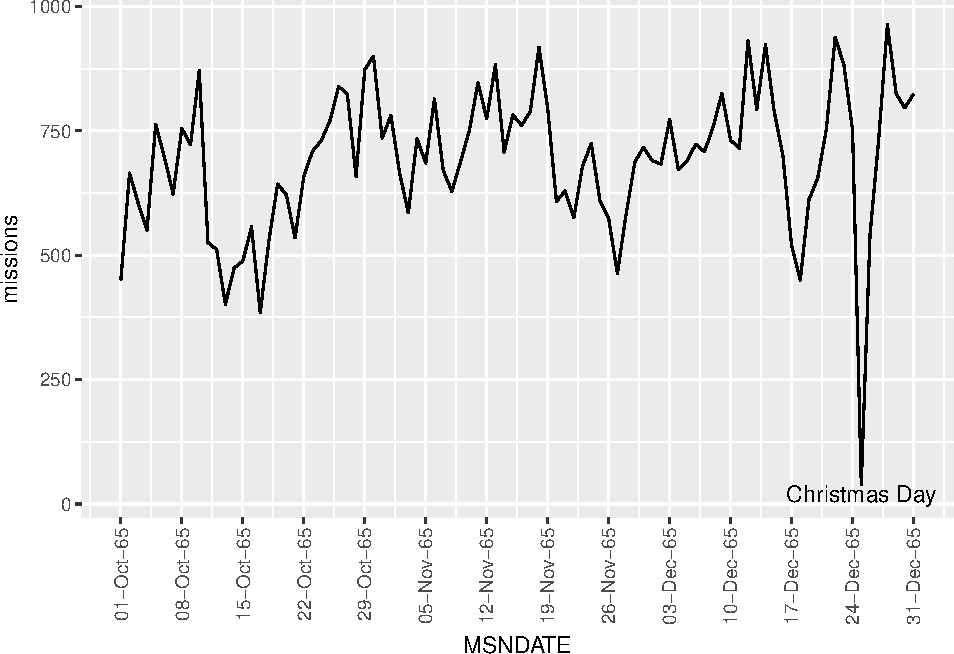
\includegraphics{visualization_files/figure-latex/unnamed-chunk-32-1.pdf}

\section{Line Width, Color, and
Points}\label{line-width-color-and-points}

We can make some adjustments to the look of a line chart.

A good reference for points and lines:
\url{http://www.cookbook-r.com/Graphs/Shapes_and_line_types/}

Let's make the following changes:

\begin{enumerate}
\def\labelenumi{\arabic{enumi}.}
\item
  Increase the width and color of the line with
  \texttt{geom\_line(size\ =\ 1,\ color\ =\ "blue")}.
\item
  Add points and change the shape and size of the point with
  \texttt{geom\_point(shape\ =\ 15,\ size\ =\ 2)}.
\end{enumerate}

\begin{Shaded}
\begin{Highlighting}[]
\KeywordTok{ggplot}\NormalTok{(msn,}\KeywordTok{aes}\NormalTok{(}\DataTypeTok{x=}\NormalTok{MSNDATE, }\DataTypeTok{y=}\NormalTok{ missions)) }\OperatorTok{+}
\StringTok{  }\KeywordTok{geom_line}\NormalTok{(}\DataTypeTok{size =} \DecValTok{1}\NormalTok{, }\DataTypeTok{color =} \StringTok{"blue"}\NormalTok{) }\OperatorTok{+}
\StringTok{  }\KeywordTok{geom_point}\NormalTok{(}\DataTypeTok{shape =} \DecValTok{15}\NormalTok{, }\DataTypeTok{size =} \DecValTok{2}\NormalTok{) }\OperatorTok{+}
\StringTok{  }\KeywordTok{scale_x_date}\NormalTok{(}\DataTypeTok{breaks=}\NormalTok{datebreaks, }\DataTypeTok{labels =} \KeywordTok{date_format}\NormalTok{(}\StringTok{"%d-%b-%y"}\NormalTok{)) }\OperatorTok{+}
\StringTok{  }\KeywordTok{theme}\NormalTok{(}\DataTypeTok{axis.text.x=}\KeywordTok{element_text}\NormalTok{(}\DataTypeTok{angle=}\DecValTok{90}\NormalTok{, }\DataTypeTok{hjust=}\DecValTok{1}\NormalTok{, }\DataTypeTok{vjust =}\NormalTok{ .}\DecValTok{5}\NormalTok{))}
\end{Highlighting}
\end{Shaded}

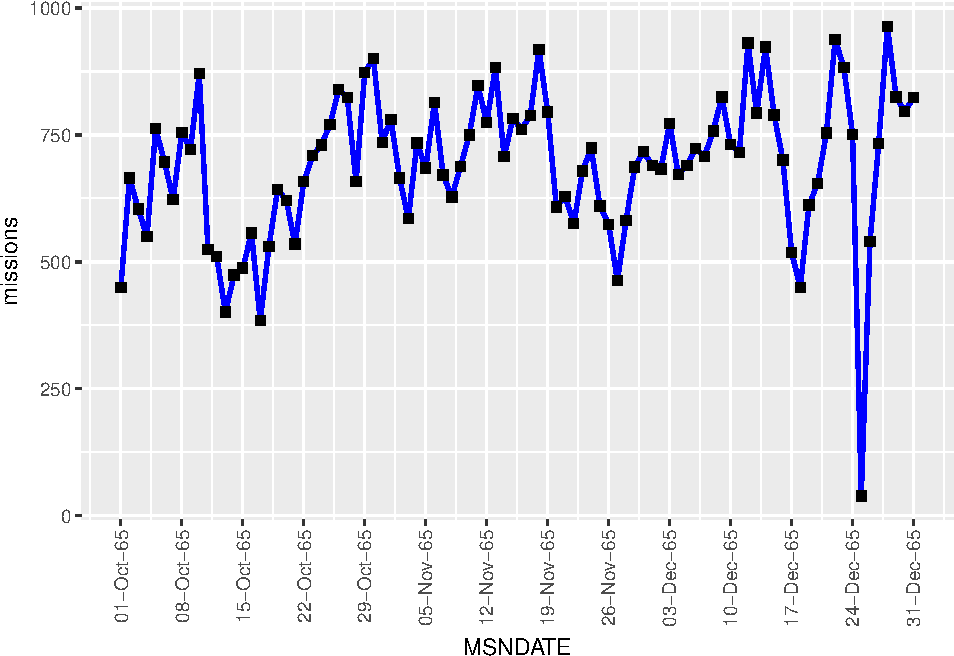
\includegraphics{visualization_files/figure-latex/unnamed-chunk-33-1.pdf}

\section{Time Series Exercise}\label{time-series-exercise}

With the mission time series chart:

\begin{enumerate}
\def\labelenumi{\arabic{enumi}.}
\item
  Use the area geom instead of line geom.
\item
  Change the points to blue and the shape to a diamond.
\item
  Add a title to the graph and center it.
\item
  Change the x-axis label to ``Date''
\item
  Change the y-axis label to ``\# of Missions''
\item
  Use ``alpha'' parameter to adjust the transparency of the area geom.
\item
  Change the fill color of the area geom to blue.
\item
  Make an annotation of ``Max Missions'' for the day with the most
  missions above the peak on the chart.
\end{enumerate}

\section{Time Series Exercise
Solution}\label{time-series-exercise-solution}

\begin{Shaded}
\begin{Highlighting}[]
\KeywordTok{ggplot}\NormalTok{(msn,}\KeywordTok{aes}\NormalTok{(}\DataTypeTok{x=}\NormalTok{MSNDATE, }\DataTypeTok{y=}\NormalTok{ missions))}\OperatorTok{+}
\StringTok{  }\KeywordTok{geom_area}\NormalTok{(}\DataTypeTok{fill=}\StringTok{'blue'}\NormalTok{,}\DataTypeTok{alpha=}\NormalTok{.}\DecValTok{3}\NormalTok{)}\OperatorTok{+}
\StringTok{  }\KeywordTok{geom_point}\NormalTok{(}\DataTypeTok{color=}\StringTok{'blue'}\NormalTok{, }\DataTypeTok{shape =} \DecValTok{5}\NormalTok{)}\OperatorTok{+}
\StringTok{  }\KeywordTok{scale_x_date}\NormalTok{(}\DataTypeTok{breaks=}\NormalTok{datebreaks, }\DataTypeTok{labels =} \KeywordTok{date_format}\NormalTok{(}\StringTok{"%d-%b-%y"}\NormalTok{)) }\OperatorTok{+}
\StringTok{  }\KeywordTok{theme}\NormalTok{(}\DataTypeTok{axis.text.x=}\KeywordTok{element_text}\NormalTok{(}\DataTypeTok{angle=}\DecValTok{90}\NormalTok{, }\DataTypeTok{hjust =} \DecValTok{1}\NormalTok{, }\DataTypeTok{vjust =}\NormalTok{ .}\DecValTok{5}\NormalTok{)) }\OperatorTok{+}
\StringTok{  }\KeywordTok{ggtitle}\NormalTok{(}\StringTok{"Number of Missions Per Day"}\NormalTok{) }\OperatorTok{+}
\StringTok{  }\KeywordTok{theme}\NormalTok{(}\DataTypeTok{plot.title =} \KeywordTok{element_text}\NormalTok{(}\DataTypeTok{hjust =}\NormalTok{ .}\DecValTok{5}\NormalTok{)) }\OperatorTok{+}
\StringTok{  }\KeywordTok{xlab}\NormalTok{(}\StringTok{"Date"}\NormalTok{) }\OperatorTok{+}
\StringTok{  }\KeywordTok{ylab}\NormalTok{(}\StringTok{'# of Missions'}\NormalTok{) }\OperatorTok{+}
\StringTok{  }\KeywordTok{annotate}\NormalTok{(}\StringTok{"text"}\NormalTok{, }\DataTypeTok{x =} \KeywordTok{as.Date}\NormalTok{(}\StringTok{"1965-12-28"}\NormalTok{), }\DataTypeTok{y =} \DecValTok{985}\NormalTok{, }\DataTypeTok{label =} \StringTok{"Max missions"}\NormalTok{)}
\end{Highlighting}
\end{Shaded}

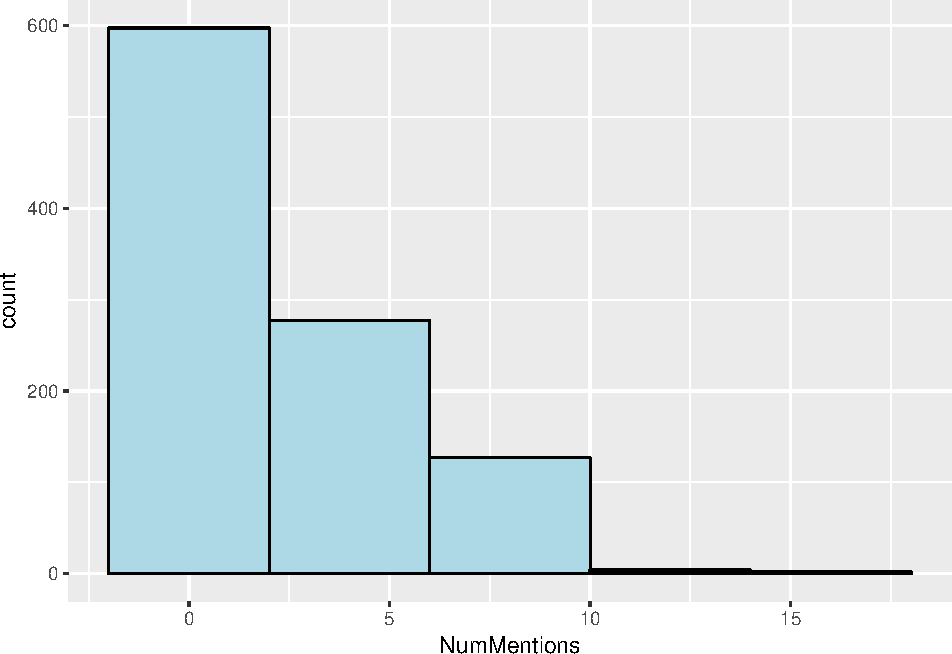
\includegraphics{visualization_files/figure-latex/unnamed-chunk-34-1.pdf}

\section{Multi-Line Charts}\label{multi-line-charts}

First, lets summarize by ``MSNDATE'' and ``TGTCOUNTRY''.

\begin{Shaded}
\begin{Highlighting}[]
\NormalTok{msn2 <-}\StringTok{ }\KeywordTok{summarise}\NormalTok{(}\KeywordTok{group_by}\NormalTok{(nam65, MSNDATE, TGTCOUNTRY), }\DataTypeTok{missions =} \KeywordTok{n}\NormalTok{())}
\KeywordTok{head}\NormalTok{(msn2)}
\end{Highlighting}
\end{Shaded}

\begin{verbatim}
## # A tibble: 6 x 3
## # Groups:   MSNDATE [2]
##      MSNDATE    TGTCOUNTRY missions
##       <date>         <chr>    <int>
## 1 1965-10-01                      1
## 2 1965-10-01          LAOS       21
## 3 1965-10-01 NORTH VIETNAM      156
## 4 1965-10-01 SOUTH VIETNAM      272
## 5 1965-10-02                      1
## 6 1965-10-02          LAOS       42
\end{verbatim}

Chart a line for each country, using the \texttt{color} aesthetic to map
to the ``TGTCOUNTRY'' variable.

\begin{Shaded}
\begin{Highlighting}[]
\KeywordTok{ggplot}\NormalTok{(msn2,}\KeywordTok{aes}\NormalTok{(}\DataTypeTok{x=}\NormalTok{MSNDATE, }\DataTypeTok{y=}\NormalTok{ missions, }\DataTypeTok{color =}\NormalTok{ TGTCOUNTRY)) }\OperatorTok{+}
\StringTok{  }\KeywordTok{geom_line}\NormalTok{() }\OperatorTok{+}
\StringTok{  }\KeywordTok{scale_x_date}\NormalTok{(}\DataTypeTok{breaks=}\NormalTok{datebreaks, }\DataTypeTok{labels =} \KeywordTok{date_format}\NormalTok{(}\StringTok{"%d-%b-%y"}\NormalTok{)) }\OperatorTok{+}
\StringTok{  }\KeywordTok{theme}\NormalTok{(}\DataTypeTok{axis.text.x=}\KeywordTok{element_text}\NormalTok{(}\DataTypeTok{angle=}\DecValTok{90}\NormalTok{, }\DataTypeTok{hjust=}\DecValTok{1}\NormalTok{, }\DataTypeTok{vjust =}\NormalTok{ .}\DecValTok{5}\NormalTok{)) }
\end{Highlighting}
\end{Shaded}

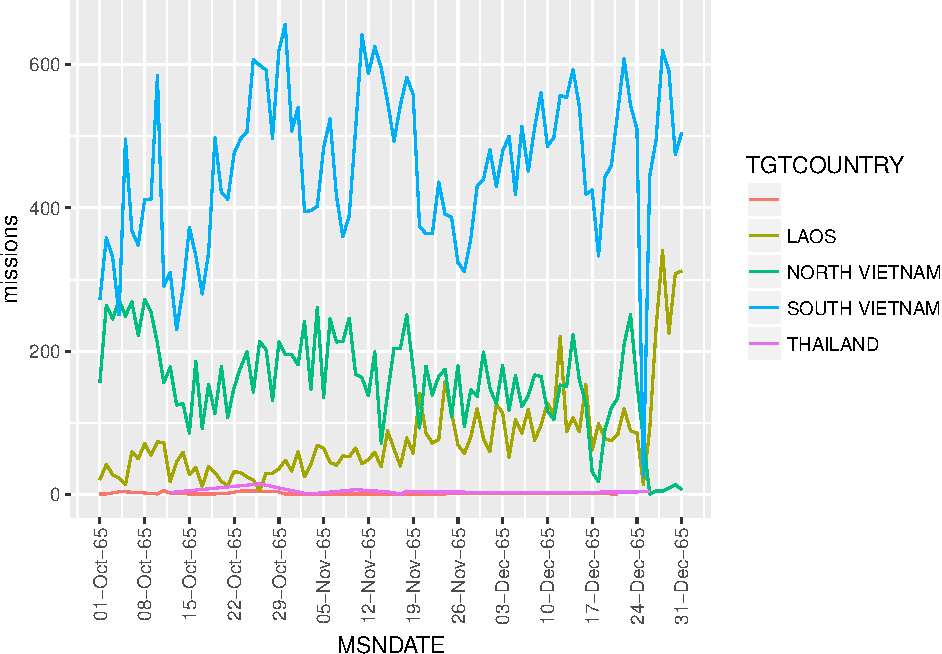
\includegraphics{visualization_files/figure-latex/unnamed-chunk-36-1.pdf}

\section{Facet Charts}\label{facet-charts}

A useful technique in data visualization is to render sub-plots of a set
of variables, as opposed to having all the variables on one plot. This
is called faceting. In this case, we will split out our multi-line chart
into a sub-plot for each target country.

\begin{itemize}
\item
  Use \texttt{facet\_grid()} or \texttt{facet\_wrap()} to plot subsets
  on separate panels.
\item
  To display sub-panels vertically, use
  \texttt{facet\_grid(TGTCOUNTRY\ \textasciitilde{}\ .)}
\item
  To display sub-panels horizontally, use
  \texttt{facet\_grid(.\ \textasciitilde{}\ TGTCOUNTRY)}
\item
  To display a sequence that wraps based on a number of rows and
  columns, use
  \texttt{facet\_wrap(\textasciitilde{}TGTCOUNTRY,\ ncol\ =\ 2)}
\end{itemize}

\begin{Shaded}
\begin{Highlighting}[]
\KeywordTok{ggplot}\NormalTok{(msn2,}\KeywordTok{aes}\NormalTok{(}\DataTypeTok{x=}\NormalTok{MSNDATE, }\DataTypeTok{y=}\NormalTok{ missions)) }\OperatorTok{+}
\StringTok{  }\KeywordTok{geom_line}\NormalTok{() }\OperatorTok{+}
\StringTok{  }\KeywordTok{facet_grid}\NormalTok{(. }\OperatorTok{~}\StringTok{ }\NormalTok{TGTCOUNTRY)}
\end{Highlighting}
\end{Shaded}

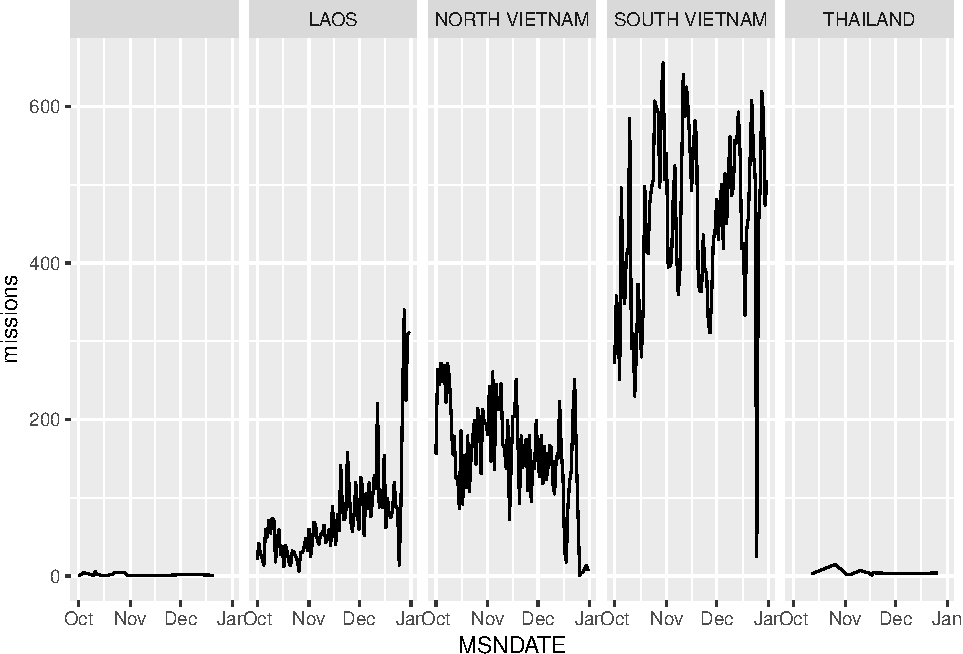
\includegraphics{visualization_files/figure-latex/unnamed-chunk-37-1.pdf}

\section{Facet Exercise}\label{facet-exercise}

Using the vietnam dataset:

\begin{enumerate}
\def\labelenumi{\arabic{enumi}.}
\item
  Create a new dataframe for number of aircraft used per operation by
  day. Hint: \texttt{summarize(group\_by())}
\item
  Replace the blanks in the OPERATIONSUPPORTED variable with ``Not
  Specified''.
\item
  Make a facet time series chart with number of aircraft on the y-axis
  and facets by operation supported.
\end{enumerate}

\section{Facet Exercise Solution}\label{facet-exercise-solution}

\begin{Shaded}
\begin{Highlighting}[]
\NormalTok{pe_facet <-}\StringTok{ }\KeywordTok{summarize}\NormalTok{(}\KeywordTok{group_by}\NormalTok{(nam65, MSNDATE, OPERATIONSUPPORTED), }\DataTypeTok{num_aircraft =} \KeywordTok{sum}\NormalTok{(NUMOFACFT))}
\NormalTok{pe_facet}\OperatorTok{$}\NormalTok{OPERATIONSUPPORTED[pe_facet}\OperatorTok{$}\NormalTok{OPERATIONSUPPORTED}\OperatorTok{==}\StringTok{""}\NormalTok{] <-}\StringTok{ "Not Specified"}
\NormalTok{datebreaks<-}\KeywordTok{seq}\NormalTok{(}\KeywordTok{as.Date}\NormalTok{(}\StringTok{"1965-10-01"}\NormalTok{),}\KeywordTok{as.Date}\NormalTok{(}\StringTok{"1965-12-31"}\NormalTok{), }\DataTypeTok{by=}\StringTok{"week"}\NormalTok{)}

\KeywordTok{ggplot}\NormalTok{(}\DataTypeTok{data =}\NormalTok{ pe_facet, }\KeywordTok{aes}\NormalTok{(}\DataTypeTok{x =}\NormalTok{ MSNDATE, }\DataTypeTok{y=}\NormalTok{num_aircraft))}\OperatorTok{+}
\StringTok{  }\KeywordTok{geom_line}\NormalTok{()}\OperatorTok{+}
\StringTok{  }\KeywordTok{scale_x_date}\NormalTok{(}\DataTypeTok{breaks=}\NormalTok{datebreaks, }\DataTypeTok{labels =} \KeywordTok{date_format}\NormalTok{(}\StringTok{"%d-%b-%y"}\NormalTok{)) }\OperatorTok{+}
\StringTok{  }\KeywordTok{theme}\NormalTok{(}\DataTypeTok{axis.text.x=}\KeywordTok{element_text}\NormalTok{(}\DataTypeTok{angle=}\DecValTok{90}\NormalTok{, }\DataTypeTok{hjust=}\DecValTok{1}\NormalTok{, }\DataTypeTok{vjust =}\NormalTok{ .}\DecValTok{5}\NormalTok{))}\OperatorTok{+}
\StringTok{  }\KeywordTok{facet_wrap}\NormalTok{(}\OperatorTok{~}\NormalTok{OPERATIONSUPPORTED, }\DataTypeTok{ncol =} \DecValTok{3}\NormalTok{)}
\end{Highlighting}
\end{Shaded}

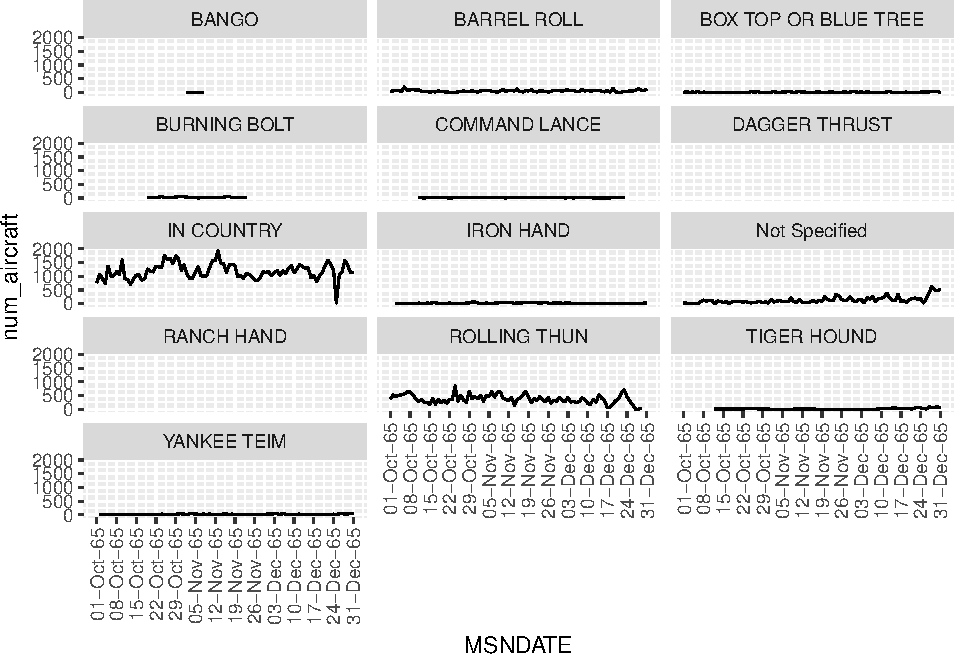
\includegraphics{visualization_files/figure-latex/unnamed-chunk-38-1.pdf}

\chapter{Histograms}\label{histograms}

A histogram is used to map a continuous variable to the x-axis and use
bins to depict the distribution of that variable.

\section{hist()}\label{hist}

Let's take a look at the distribution of missions by time of day based
on the ``TIMEONTARGET'' variable.

Base R has a simple histogram function, \texttt{hist()}.

\begin{Shaded}
\begin{Highlighting}[]
\KeywordTok{hist}\NormalTok{(nam65}\OperatorTok{$}\NormalTok{TIMEONTARGET)}
\end{Highlighting}
\end{Shaded}

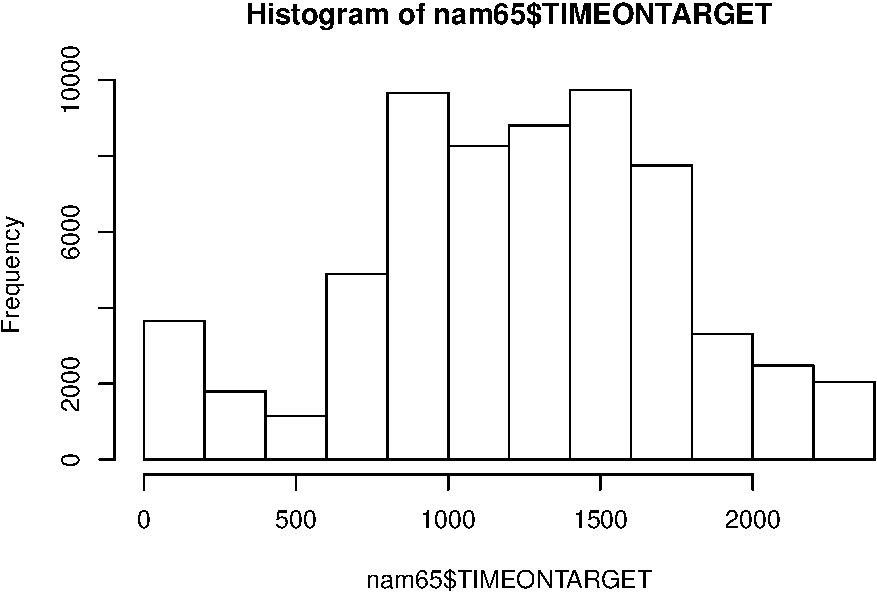
\includegraphics{visualization_files/figure-latex/unnamed-chunk-39-1.pdf}

We can adjust the number of bins with the ``breaks'' parameter.

\begin{Shaded}
\begin{Highlighting}[]
\KeywordTok{hist}\NormalTok{(nam65}\OperatorTok{$}\NormalTok{TIMEONTARGET, }\DataTypeTok{breaks =} \DecValTok{24}\NormalTok{)}
\end{Highlighting}
\end{Shaded}

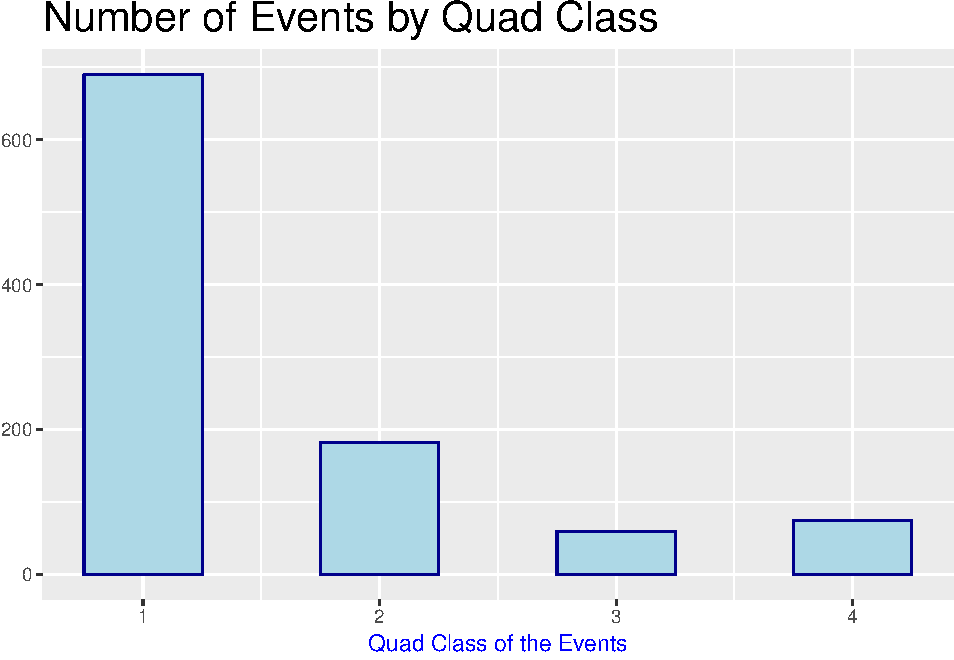
\includegraphics{visualization_files/figure-latex/unnamed-chunk-40-1.pdf}

\section{geom\_histogram()}\label{geom_histogram}

But if we want to apply the customization and other techniques we've
learned to this plot, we need to use \textbf{ggplot2}.

In \textbf{ggplot2}, the geom for histograms is:
\texttt{geom\_histogram()}.

Here's a basic histogram with \textbf{ggplot2}:

\begin{Shaded}
\begin{Highlighting}[]
\KeywordTok{ggplot}\NormalTok{(}\DataTypeTok{data =}\NormalTok{ nam65, }\KeywordTok{aes}\NormalTok{(}\DataTypeTok{x =}\NormalTok{ TIMEONTARGET)) }\OperatorTok{+}
\StringTok{  }\KeywordTok{geom_histogram}\NormalTok{()}
\end{Highlighting}
\end{Shaded}

\begin{verbatim}
## `stat_bin()` using `bins = 30`. Pick better value with `binwidth`.
\end{verbatim}

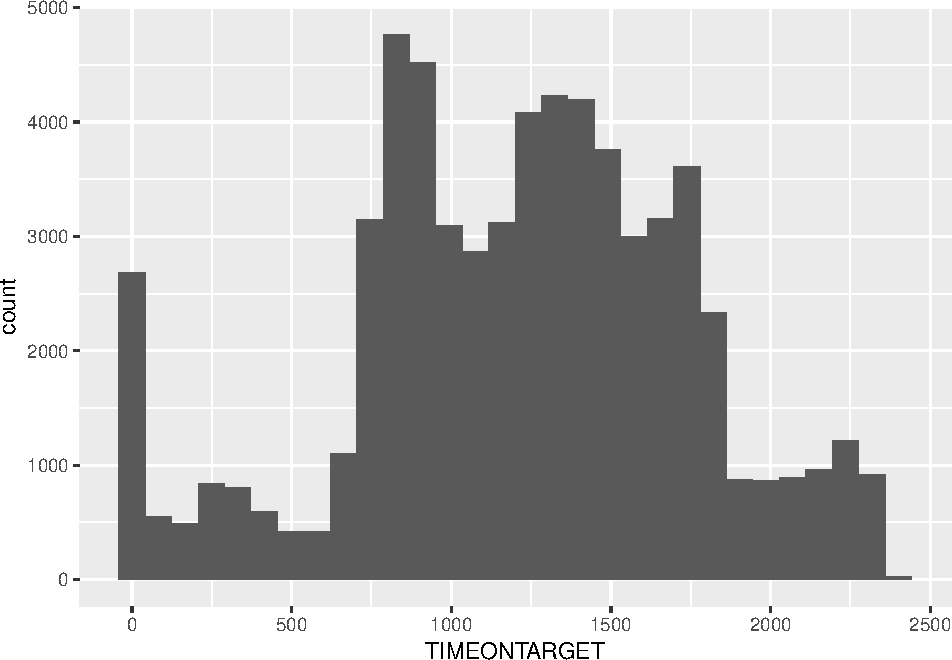
\includegraphics{visualization_files/figure-latex/unnamed-chunk-41-1.pdf}

\section{Bins}\label{bins}

The default in \textbf{ggplot} is 30 bins. But we can set the number of
bins in two ways.

First, we can change the width of the bin.

\begin{itemize}
\item
  Use ``100'' as the binwidth to approximate an hour.
\item
  We will also adjust the fill and border colors to make the graph
  easier to read.
\end{itemize}

\begin{Shaded}
\begin{Highlighting}[]
\KeywordTok{ggplot}\NormalTok{(}\DataTypeTok{data =}\NormalTok{ nam65, }\KeywordTok{aes}\NormalTok{(}\DataTypeTok{x =}\NormalTok{ TIMEONTARGET)) }\OperatorTok{+}
\StringTok{  }\KeywordTok{geom_histogram}\NormalTok{(}\DataTypeTok{binwidth =} \DecValTok{100}\NormalTok{, }\DataTypeTok{fill =} \StringTok{"lightblue"}\NormalTok{, }\DataTypeTok{color =} \StringTok{"black"}\NormalTok{)}
\end{Highlighting}
\end{Shaded}

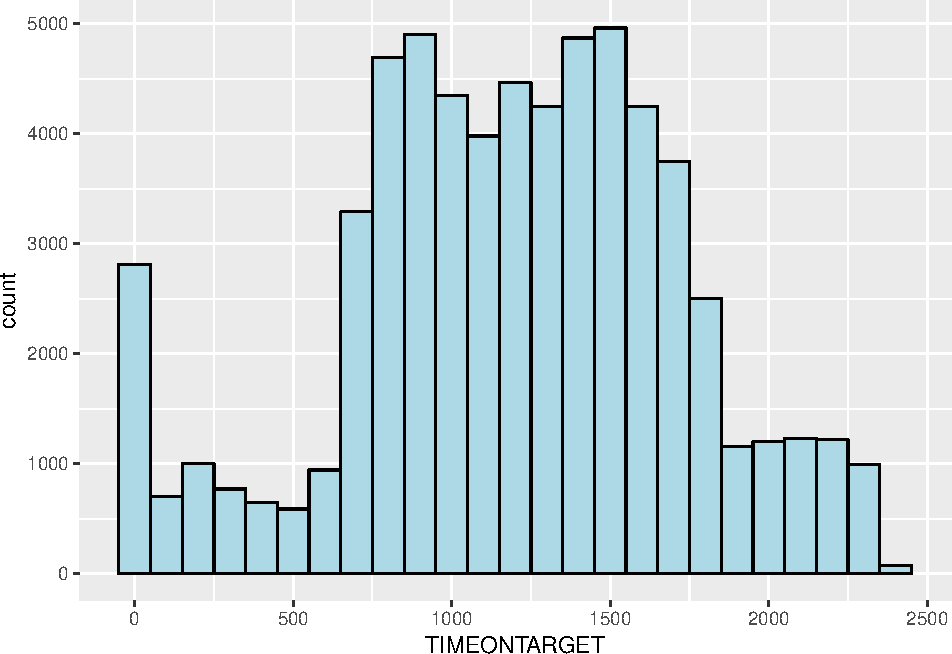
\includegraphics{visualization_files/figure-latex/unnamed-chunk-42-1.pdf}

Another option is to set the number of bins with the ``bins'' parameter.

\begin{Shaded}
\begin{Highlighting}[]
\KeywordTok{ggplot}\NormalTok{(}\DataTypeTok{data =}\NormalTok{ nam65, }\KeywordTok{aes}\NormalTok{(}\DataTypeTok{x =}\NormalTok{ TIMEONTARGET)) }\OperatorTok{+}
\StringTok{  }\KeywordTok{geom_histogram}\NormalTok{(}\DataTypeTok{bins =} \DecValTok{24}\NormalTok{, }\DataTypeTok{fill =} \StringTok{"pink"}\NormalTok{, }\DataTypeTok{color =} \StringTok{"black"}\NormalTok{)}
\end{Highlighting}
\end{Shaded}

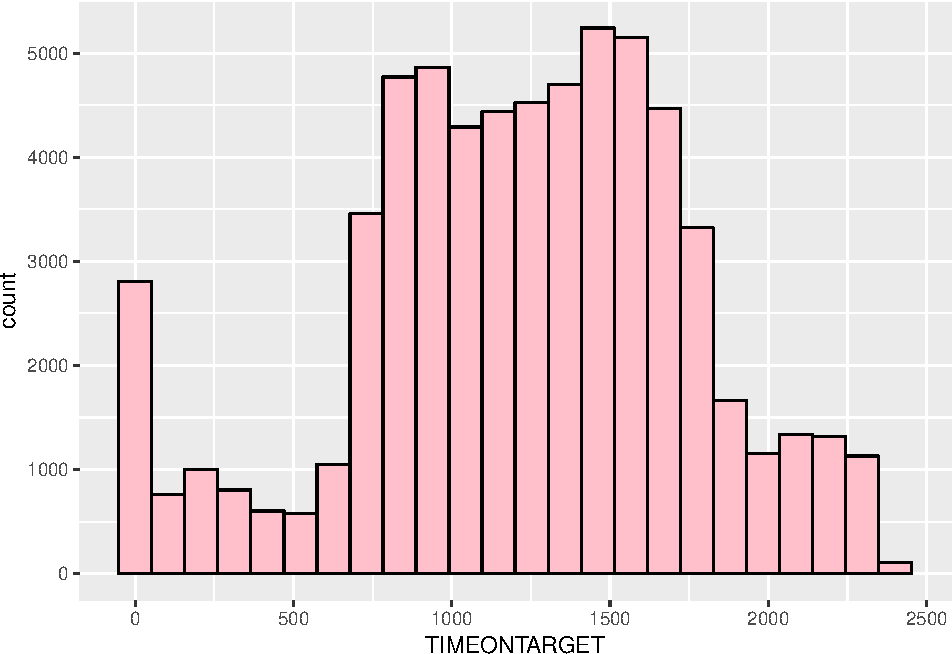
\includegraphics{visualization_files/figure-latex/unnamed-chunk-43-1.pdf}

\section{Histogram Exercise}\label{histogram-exercise}

\begin{enumerate}
\def\labelenumi{\arabic{enumi}.}
\item
  Build a histogram for the distribution of missions per day. Hint: set
  the bins equal to the number of days in the dataset.
\item
  Make the color of the bars light blue and the outline of the bars navy
  blue.
\end{enumerate}

\section{Histogram Exercise Solution}\label{histogram-exercise-solution}

\begin{Shaded}
\begin{Highlighting}[]
\KeywordTok{ggplot}\NormalTok{(}\DataTypeTok{data =}\NormalTok{ nam65, }\KeywordTok{aes}\NormalTok{(}\DataTypeTok{x =}\NormalTok{ MSNDATE))}\OperatorTok{+}
\StringTok{  }\KeywordTok{geom_histogram}\NormalTok{(}\DataTypeTok{bins =} \DecValTok{92}\NormalTok{, }\DataTypeTok{fill =} \StringTok{"lightblue"}\NormalTok{, }\DataTypeTok{color =} \StringTok{"blue"}\NormalTok{)}
\end{Highlighting}
\end{Shaded}

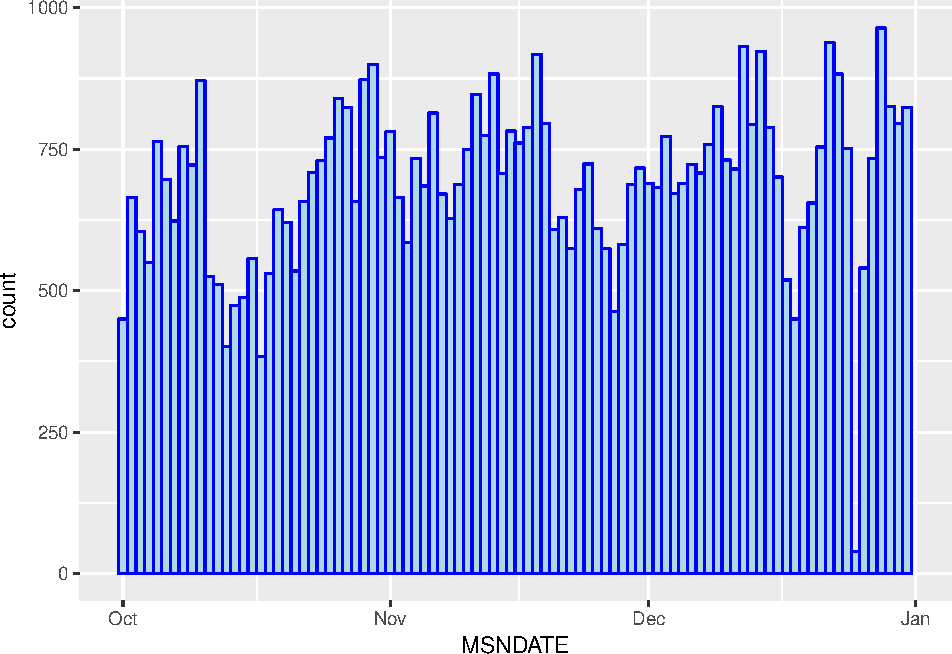
\includegraphics{visualization_files/figure-latex/unnamed-chunk-44-1.pdf}

\chapter{Interactive Graphics}\label{interactive-graphics}

You can create interactive graphics with the \textbf{plotly} package.

\begin{itemize}
\item
  Plotly works as a wrapper around charts made in base R or ggplot.
\item
  Create an object with your ggplot code, then use \texttt{ggplotly()}
  to convert the plot.
\end{itemize}

\begin{Shaded}
\begin{Highlighting}[]
\NormalTok{g <-}\StringTok{ }\KeywordTok{ggplot}\NormalTok{(msn2,}\KeywordTok{aes}\NormalTok{(}\DataTypeTok{x=}\NormalTok{MSNDATE, }\DataTypeTok{y=}\NormalTok{ missions, }\DataTypeTok{color =}\NormalTok{ TGTCOUNTRY)) }\OperatorTok{+}
\StringTok{  }\KeywordTok{geom_line}\NormalTok{()}\OperatorTok{+}
\StringTok{  }\KeywordTok{scale_x_date}\NormalTok{(}\DataTypeTok{breaks=}\NormalTok{datebreaks, }\DataTypeTok{labels =} \KeywordTok{date_format}\NormalTok{(}\StringTok{"%d-%b-%y"}\NormalTok{)) }\OperatorTok{+}
\StringTok{  }\KeywordTok{theme}\NormalTok{(}\DataTypeTok{axis.text.x=}\KeywordTok{element_text}\NormalTok{(}\DataTypeTok{angle=}\DecValTok{90}\NormalTok{, }\DataTypeTok{hjust=}\DecValTok{1}\NormalTok{, }\DataTypeTok{vjust =}\NormalTok{ .}\DecValTok{5}\NormalTok{))}

\KeywordTok{ggplotly}\NormalTok{(g)}
\end{Highlighting}
\end{Shaded}


\end{document}
